\documentclass{article}	
%\usepackage{times}
\usepackage{amsmath}
\usepackage{graphicx}
\usepackage{myapalike}
\usepackage{tabularx}

%\renewcommand{\rmdefault}{phv}
%\renewcommand{\ttdefault}{phv}

\hoffset-2cm
\addtolength{\textwidth}{3cm}
%\voffset-1cm
\addtolength{\textheight}{2cm}

\makeatletter
\newenvironment{myenum}{
% \renewcommand{\theenumi}{\roman{enumi}}
% \renewcommand{\labelenumi}{(\theenumi)}
\begin{list}{\labelenumi}{\setlength{\leftmargin}{1.3em}
  \setcounter{enumi}{0}
  \renewcommand{\item}{\addtocounter{enumi}{1}\unskip \vspace{-0.1cm}\@inmatherr\item
  \@ifnextchar [\@item{\@noitemargtrue \@item[\@itemlabel]} \unskip}}
  \itemsep0.1cm plus0.1cm minus0.05cm
  \listparindent0cm
  \setlength{\labelsep}{0.5em}
  \setlength{\labelwidth}{0.8em}}
{\end{list}}
\makeatother

\newenvironment{myitem}{\begin{list}{$\bullet$}{\setlength{\leftmargin}{1.1em}
\itemsep0.1cm plus0.1cm minus0.05cm
\listparindent0cm
\addtolength{\labelsep}{0.5\labelsep}
\setlength{\labelwidth}{0.8em}
\setlength{\leftmargin}{\labelwidth}
\addtolength{\leftmargin}{\labelsep}
}}{\end{list}}


\begin{document}

\begin{titlepage}
  \begin{center}
  {{\bf \Large 
    StdpC 7.1 }\\[0.3cm]
    \large (Spike timing dependent plasticity Clamp)}, \\[1cm]
  {\large 
    in parts based on {\bf DYNCLAMP2} \cite{Pinto2001} 
  } \\[2cm]
  {\sc \Large Manual }
  \end{center}
\vspace*{2cm}

\noindent
{\large Thomas Nowotny} \\[0.5cm]
Centre for Computational Neuroscience and Robotics, \\
School of Engineering and Informatics, \\
University of Sussex, \\
Brighton BN1 9QJ, UK \\
E-mail: t.nowotny@sussex.ac.uk
 \\[1cm]
{\large Felix B. Kern} \\[0.5cm]
School of Life Sciences, \\
University of Sussex, \\
Brighton BN1 9QG, UK
 \\[1cm]
Original DYNCLAMP2 developers: \\[0.2cm]
Reynaldo Daniel Pinto, \\
Robert C. Elson, \\
Attila Sz\"ucs, \\
M. I. Rabinovich, \\
A. I. Selverston,  \\
H. D. I. Abarbanel \\[0.5cm]
Institute for Nonlinear Science, \\
University of California, San Diego, \\
9500 Gilman Dr. \\ Mail Code 0402 \\
La Jolla, CA 92093-0402, USA \\

\end{titlepage}

StdpC is software building on the ideas that led
to the development of the earlier DYNCLAMP2
software. The new software is based on Qt and comes in two versions, one
for the old DigiData 1200/A interface, the other supporting all National
Instruments devices that support NI's NIDAQmx API.
 
Some functionality in this software has
not been tested thoroughly. Any feedback on problems with the
software or potential bugs is greatly appreciated.  Older versions
of the software (StdpC) are described in Journal of Neuroscience
Methods \cite{Nowotny2006} and, more recently, in Nature Protocols 
\cite{Kemenes2011}. {\em If you use StdpC and publish results
based on its use, please cite the website and these papers.} Please
contact us for any further questions (t.nowotny@sussex.ac.uk).

Copyright 2019 T.~Nowotny \& F.~B.~Kern

StdpC is free software; you can redistribute it and/or modify  
it under the terms of the GNU General Public License as published by 
the Free Software Foundation; either version 2 of the License, or 
(at your option) any later version.                               

This program is distributed in the hope that it will be useful,
but WITHOUT ANY WARRANTY; without even the implied warranty of
MERCHANTABILITY or FITNESS FOR A PARTICULAR PURPOSE.  See the 
GNU General Public License for more details.

You should have received a copy of the GNU General Public License
along with this program; if not, write to the
Free Software Foundation, Inc., 59 Temple Place - Suite 330, Boston,
MA  02111-1307, USA.

\newpage
\section{Introduction}
           
The Dynamic Clamp protocol, developed by \cite{Sharp1993} and
independently by \cite{Robinson1993} allows inserting simulated
membrane conductances into cells, and/or adding synapses between cells
as well as a variety of other manipulations. Here, we describe StdpC
2019, a software for controlling biological neurons and an internal
spike generator in (soft) real time.

The software allows its user to define artificial synapses, Hodgkin-Huxley conductances
\cite{Hodgkin1949}, simulated neurons built from such conductances, and
presynaptic spike generators. The parameters of these simulated
entities can be controlled on the graphical user interface (GUI) or
through script files.  

StdpC has a built in electrode compensation method (Active
Electrode Compensation \cite{Brette2008}), which is optionally usable after
going through a short and automatic calibration procedure. This
compensation technique allows for application of a single electrode both
for stimulation and recording with higher signal fidelity than conventional
compensation techniques, like bridge balancing or discontinuous
injection/recording. 

During the experiment, the acquired data can be saved continuously into a
data file either in ASCII or binary format for off-line post-processing and
results analysis.
 
The software supports the DIGIDATA 1200A data acquisition card of Axon
Instruments, Inc (now part of MDS Analytical Technologies), all
NIDAQmx capable devices of National Instruments, and a pure simulation
mode for testing. The program was written in C++ (using
QtCreator). The graphical user interface is based on Qt
libraries. The program has been developed and tested on Windows 7 but should also
be compatible with newer versions up to Windows 10. StdpC may or may not work on
older versions of Windows, subject particularly to the DIGIDATA and NIDAQmx drivers.
Newer DIGIDATA versions are currently not supported; please contact us if you
wish to change this.

\section{Hardware and software requirements} 
 
A standard PC, Windows 7-10 (older versions of Windows may work, but are untested).
A DIGIDATA 1200A ADC/DAC board from Axon
Instruments, or a National Instruments DAQ and installed NIDAQmx
driver.

The program was tested on a PC with Windows 7 Professional and a
National Instruments PCIe-6251 DAQ using NIDAQmx for
Windows, version 18.5.

\section{Asynchronous Dynamic Clamp Cycle}
 
The dynamic clamp protocol consists of a cycle of reading the membrane
potential of the cells, calculating the current to be injected into
the cells according to the synapses and conductances that are to be
simulated, and generating the voltage commands that will generate the
currents. StdpC aims at repeating this cycle at the maximal rate
supported by the hardware in order to simulate continuous biological
processes. Since Windows is not a real time operating system, the
actual time from one cycle to the next can not be controlled in a
strict way. Instead of aiming at such a control StdpC is based on an
asynchronous dynamic clamp cycle.  Every time the program updates the
membrane potential of the cells it also reads the system clock,
which allows it to calculate the duration of the previous
Dynamic Clamp cycle. The measured time intervals between voltage
updates are used in the computation of the currents. This limits the
impact of unequal delays during repeated cycles unless these delays
become large compared to the biological time scales in the system
studied. As a side effect of the asynchronous Dynamic Clamp cycle,
StdpC update cycles will always run at the maximum rate supported by
the hardware. With the typical successive upgrade of computer hardware
the quality of the Dynamic Clamp interaction will improve over time.


\section{How to install the software}

\subsection{Precompiled executables}
Download the exe file to a convenient location, e.g.,
C:$\backslash$Program Files$\backslash$StdpC.exe and execute.

\subsection{Source package}
Download the source package and unzip it to a convenient
location, or check it out via git. To build StdpC from source, you will need Qt 5 
and either the msvc toolchain (recommended) or mingw (if you require Digidata 1200/A support).
We recommend compiling from within QtCreator, but you may find it more convenient to invoke
qmake.exe from a shell instead. You can control driver support by adding ``nidaqmx'',
``nonidaqmx'' or ``digidata'' to the CONFIG environment variable 
(e.g. ``qmake.exe [...] CONFIG+=nidaqmx'').

\section{Troubleshooting}
\subsection{I/O conflicts}
 
In the past, there have been problems with I/O conflicts between the
DigiData board and other hardware devices. If you are experiencing
problems, you may need to change the base address of the DigiData
board. Hardware conflicts can occur even if the DIGIDATA board works
fine with Axon programs like Axoscope because, unlike these, StdpC
2017 does read the Real Time Counter (RTC) in the Digidata
board. Usually, the DigiData board is configured to use the I/O base
address 0x320, and in this case the RTC reading ports are in the range
of 0x330 - 0x332. Many computers use the address 0x330 for some devices like
sound cards, etc.

To check for and resolve a hardware address conflict,
\noindent
{\em Windows NT, 2000, XP: } \\
Open: Start $\rightarrow$ Programs $\rightarrow$ Administrative Tools
$\rightarrow$ Windows NT Diagnostics. Choose the folder
$\langle$Resources$\rangle$, click in $\langle$I/O Port$\rangle$ and use the
cursor to browse the list of used ports.  You should look for 330. Note that
320 will not appear because the Digidata Board is not detected by Windows. If
you find any reference in the range 330 - 33F and your Digidata board is
configured to use the base address 320 you need to change I/O address of your
Digidata board to run StdpC and avoid other problems due to the I/O
conflict.

\noindent
{\em Windows 95, 98: } \\ Open: Start $\rightarrow$ Settings
$\rightarrow$ Control Panel $\rightarrow$ System. Choose the folder
$\langle$Device Manager$\rangle$, click $\langle$I/O Port$\rangle$ and
use the cursor to browse the list of used ports. You should look for
330.  Note that 320 will not appear because the Digidata Board is not
detected by Windows. If you find any reference in the range 330 - 33F
and your Digidata board is configured to use the base address 320 you
need to change the I/O address of your Digidata board to run StdpC
and avoid other problems due to the I/O conflict.
 
\noindent
{\em Changing the base address of the Digidata Board and in the StdpC
  program: } \\ Identify a free range of port addresses.  If 0x330 is
in use, addresses around 340-370 are usually available which is
sufficient for the Digidata ports. Reconfigure the Digidata
board for the base address 340 or 350 manually (the RTC will be 350 or
360 and no conflicts!) and run the StdpC program. The Digidata base
address can be changed within StdpC on the Digidata settings dialog.

\section{Changes from previous versions/programs}
\subsection{Changes DYNCLAMP2 to StdpC version 3}
The following is a list of features which were new in StdpC v3: 
\begin{myitem}
  \item {\em Spike generator} \\
    A spike generator can replace a biological presynaptic neuron. Spikes are
    generated either periodically in a fixed pattern or from a file
    containing predefined spike times. This feature is actually an original
    feature of R. Pinto but was not published yet.
  \item {\em Hidden parameter panels} \\
    To de-clutter the screen of the dynamic clamp computer, in StdpC the
    parameter dialogs for chemical synapses and Hodgkin-Huxley conductances
    have been moved to separate pop-up windows.
  \item {\em Data displays for debugging} \\
    To allow for easy debugging of wiring and gain problems the software now
    has two data displays that can show input and/ or output channels or
    functions thereof (averages, spikes detected).
  \item {\em Save and load parameter settings} \\
    You can now save and load the current parameter settings of the
    clamp. This way one does not have to redo parameter settings every time
    the StdpC program is restarted. The settings are stored in a simple ASCII
    format that allows editing by hand or snooping around for curiosity. 
  \item {\em Spike timing dependent plasticity} \\
    The two chemical synapses can now be made plastic obeying a Spike Timing
    Dependent Plasticity protocol. There are two different protocols to
    choose from and a variety of parameters determining the details of the
    learning mechanism
  \item {\em Experimental automatization and scripting} \\
    The StdpC supports a simple form of experimental protocol automation
    (scripting). The user can specify a script file that contains events at
    given times. These events include switching on and off of synaptic
    connections or Hodgkin-Huxley type conductances as well as arbitrary
    parameter changes. The script is loaded on starting the clamping process
    and executes the commands at the given times after clamping started.
\end{myitem}

\subsection{Changes from StdpC version 3 to version 4}
\begin{myitem}
\item Since this version of StdpC, all synapses are freely reconfigurable as
  chemical or electrical synapses.
\item the presynaptic and postsynaptic neuron of each synapse is freely
  reconfigurable. In particular it is now possible to combine synapses
  between two biological neurons (on channels IN0/OUT0  and IN1/OUT1) with
  synapses from 
  the spike generator (channel SPG) to either of the neurons. This gives more
  flexibility in the experimental design
\item Each chemical synapse can now been chosen individually to be plastic or not.
\item The initial value for a plastic synapse is given by its individual G\_s
  setting, not by a global initialisation value in the plasticity block. The
  displays for the synaptic strength have been removed because they turned
  out to be disruptive for the clamping performance.
\item Some smaller adjustments aiming at better user interaction and
  performance of the data displays. We, however, still recommend not to use
  the data displays during real experiments. They are for debugging purposes
  only and degrade clamping performance considerably when used.
\end{myitem}

\subsection{Changes from StdpC v4 to StdpC 2007 (v5)}
\begin{myitem}
\item The user interface is now based on QT
\item The driver for the DigiData 1200 board was re-created using (an
  extended version of) the free PortTalk package.
\item StdpC 2007 supports all NIDAQmx capable National Instruments boards
\item The source code has been re-organised to allow for rapid
  inclusion of additional hardware support.
\item StdpC 2007 allows to use all input and output channels available
  on the acquisition hardware.
\item All synaptic properties including the details of the synaptic
  plasticity are now individually adjustable for every synapse
\item There are now two alternative descriptions for Hodgkin-Huxley
  type conductances, including several functional forms for the
  activation and inactivation curves.
\item With the additional support for other hardware, there is now
  more fine-grained control over the channels that are used for
  voltage and current conversion. All channels are available in
  ``input channels'' and ``output channels'' dialogs. Only channels
  activated in these dialogs will appear in the drop-down menus within
  synapses and HH conductances.
\end{myitem}

\subsection{Changes from StdpC 2007 to StdpC 2010 (v6.0)}
\begin{myitem}
\item Active Electrode Compensation feature included as an optional,
  automatic, digital electrode compensation technique calculated within the
  software.                  
\item A new feature allows for the measurement of the resistance and
  capacitance properties of both the electrode and cell membrane,
  conveniently controlled from the software.  
\item Full experimental data saving support has been included. Any
  combination of the active input and output channels, along with the spike generator, can
  be saved, with a frequency (quasi) independent of the main dynamic clamp
  loop frequency. Data can be saved either in ASCII, or in binary format.
\item A constant bias current can now be defined for any active output
  channel for special experiment configuration needs. 
\end{myitem}

\subsection{Changes from StdpC 2010 to StdpC 2011 (v6.1)}
\begin{myitem}
\item Active electrode compensation is now stable.
\item Through scripting, a sample-and-hold mechanism can be envoked if
  measurement artefacts due to the experimental protocol need to be
  removed from voltage signals. For example, the monitoring of
  membrane potentials can be interrupted during stimulation from
  sources external to the dynamic clamp.
\item The synapse models have been updated with the addition of the
  ``Destexhe synapse'' and a modification of the alph-beta synapse.
\item A variety of minor bugs and issues have been fixed.
\item Data saving can now be enabled and disabled globally in teh data
  saving dialog. This overrides the choices for individual channels,
  and if disabled, the overheads of this mechanism can be avoided.
\end{myitem}

\subsection{Changes from StdpC 2012 to StdpC 2017 (v7.0)}
\begin{myitem}
\item m/h/tau HH currents received two new tau formulations.
\item AEC computed currents can now be directed to a separate channel for data output
 purposes in addition to its usual function. In addition, there is no longer any restriction
 on the number of AEC channels.
\item It is now possible to use several data sources (DAQs, files, spike generators, models) simultaneously.
\item There is now an option to simulate entire (single-compartment) Hodgkin-Huxley neurons, see
 section \ref{HHmodels} for details.
\item It is now possible to define an arbitrary number of HH conductances and synapses.
\item Currents and synapses can now be assigned to more than one set of channels.
 Each assignment draws on the common parameter set, but is functionally independent
 from other assignments. As a consequence of this update, the channel assignments
 in protocols and scripts written for/by older StdpC versions may be wrongly converted.
 Please check for correctness and/or update your scripts and protocols, see section \ref{scriptsect} for details.
\item Synapses (but not gap junctions) now support conduction delays.
\item Currents, synapses, channel assignments, neuron models and model instances can now all be
 turned on or off by script while the clamp cycle is running, provided that they were active when
 the clamp cycle was started.
\item Graph performance and handling has been improved.
\item A performance indicator has been added to the main window showing the actual clamp cycle
frequency.
\item Large parts of the code have been cleaned up and refactored/rewritten into a more modular design.
\end{myitem}

\subsection{Changes from StdpC 2017 to StdpC 7.1}
\begin{myitem}
\item The clamp thread's priority can now be set by the user to trade off between maximum performance
and the threat of potentially freezing one's system.
\item The clamp cycle can now be started after a settling period, or by way of a digital trigger input.
\item A new data source was added, Voltage Stepper, which produces square steps.
\item Several tools were added, including a generator pseudo-random synaptic background noise, a
``wire'' facility to pass data from input to output channels, and an experimental software-defined
voltage clamp using PID control.
\item The chemical synapse model can now produce stochastically sized post-synaptic potentials.
\item Synaptic gSyn can now be multiplied with samples from an input channel, e.g. from SimulDAQ input.
\item Data saving has become much more flexible, both in terms of output format and in terms of the naming
of the output file(s).
\item The GUI has received numerous upgrades and improvements to usability.
\item We have added MSVC build capability. The MSVC build runs faster, but does not support the Digidata
driver. For Digidata 1200/A users, a mingw build is still provided.
\item A number of bugs have been fixed.
\end{myitem}

\section{How to use StdpC}

\subsection{``Connecting'' the program to the cells}
 
To avoid the generation of wrong current commands due to artifacts
introduced into the membrane measurement by the current injection,
one must either (1) insert of two electrodes into each cell (one for
injection, the other one for recording), or
(2) use a careful compensation of a single electrode in order to recover the
actual membrane potential from the raw artefactual voltage. For the
latter solution StdpC has a built-in artifact compensation method, AEC
(Active Electrode Compensation \cite{Brette2008}), that allows for a
convenient, software-based electrode compensation. One can think of
special experiment configurations, like simultaneously recording in multiple
machines, in which AEC might not be found appropriate for compensation. In
these cases any external analogue technique like microelectrode amplifier 
features could
be applied instead of (and NOT in conjunction with) AEC. However, we
generally encourage the application of AEC, as it is an automatic method
that provides high quality signals at arbitrarily high time resolution.
See section \ref{eleccomp} for more detail about electrode compensation.

The membrane potential output of the microelectrode amplifiers should
be connected to the analog input channels chosen to be scanned in the
``input channels'' dialog. The command voltage for the injection of
current into the cells will be applied to the analog output channels chosen in
the corresponding drop-down boxes. For specific channels to appear in
these boxes, they need to be activated in the ``output channels''
dialog, and the data source they belong to must be activated.

The currents are calculated individually for each active conductance and
synapse and then are summed for each cell to generate the
corresponding voltage command for the microelectrode amplifiers. It is
recommended to turn on the dynamic clamp cycle and to monitor the
current command voltage in an oscilloscope before turning on the
injection of the current in the microelectrode amplifier, to see if it
looks like what is expected. If it is orders of magnitude wrong, check
the conversion factors in the ``input channels'' and ``output
channels'' dialogs. Alternatively, the channel setup settings can be checked and
corrected safely on a model cell, which are usually shipped with the
microelectrode amplifiers.

 
\subsection{Control Panel of the Program}

\parbox{\textwidth}{
  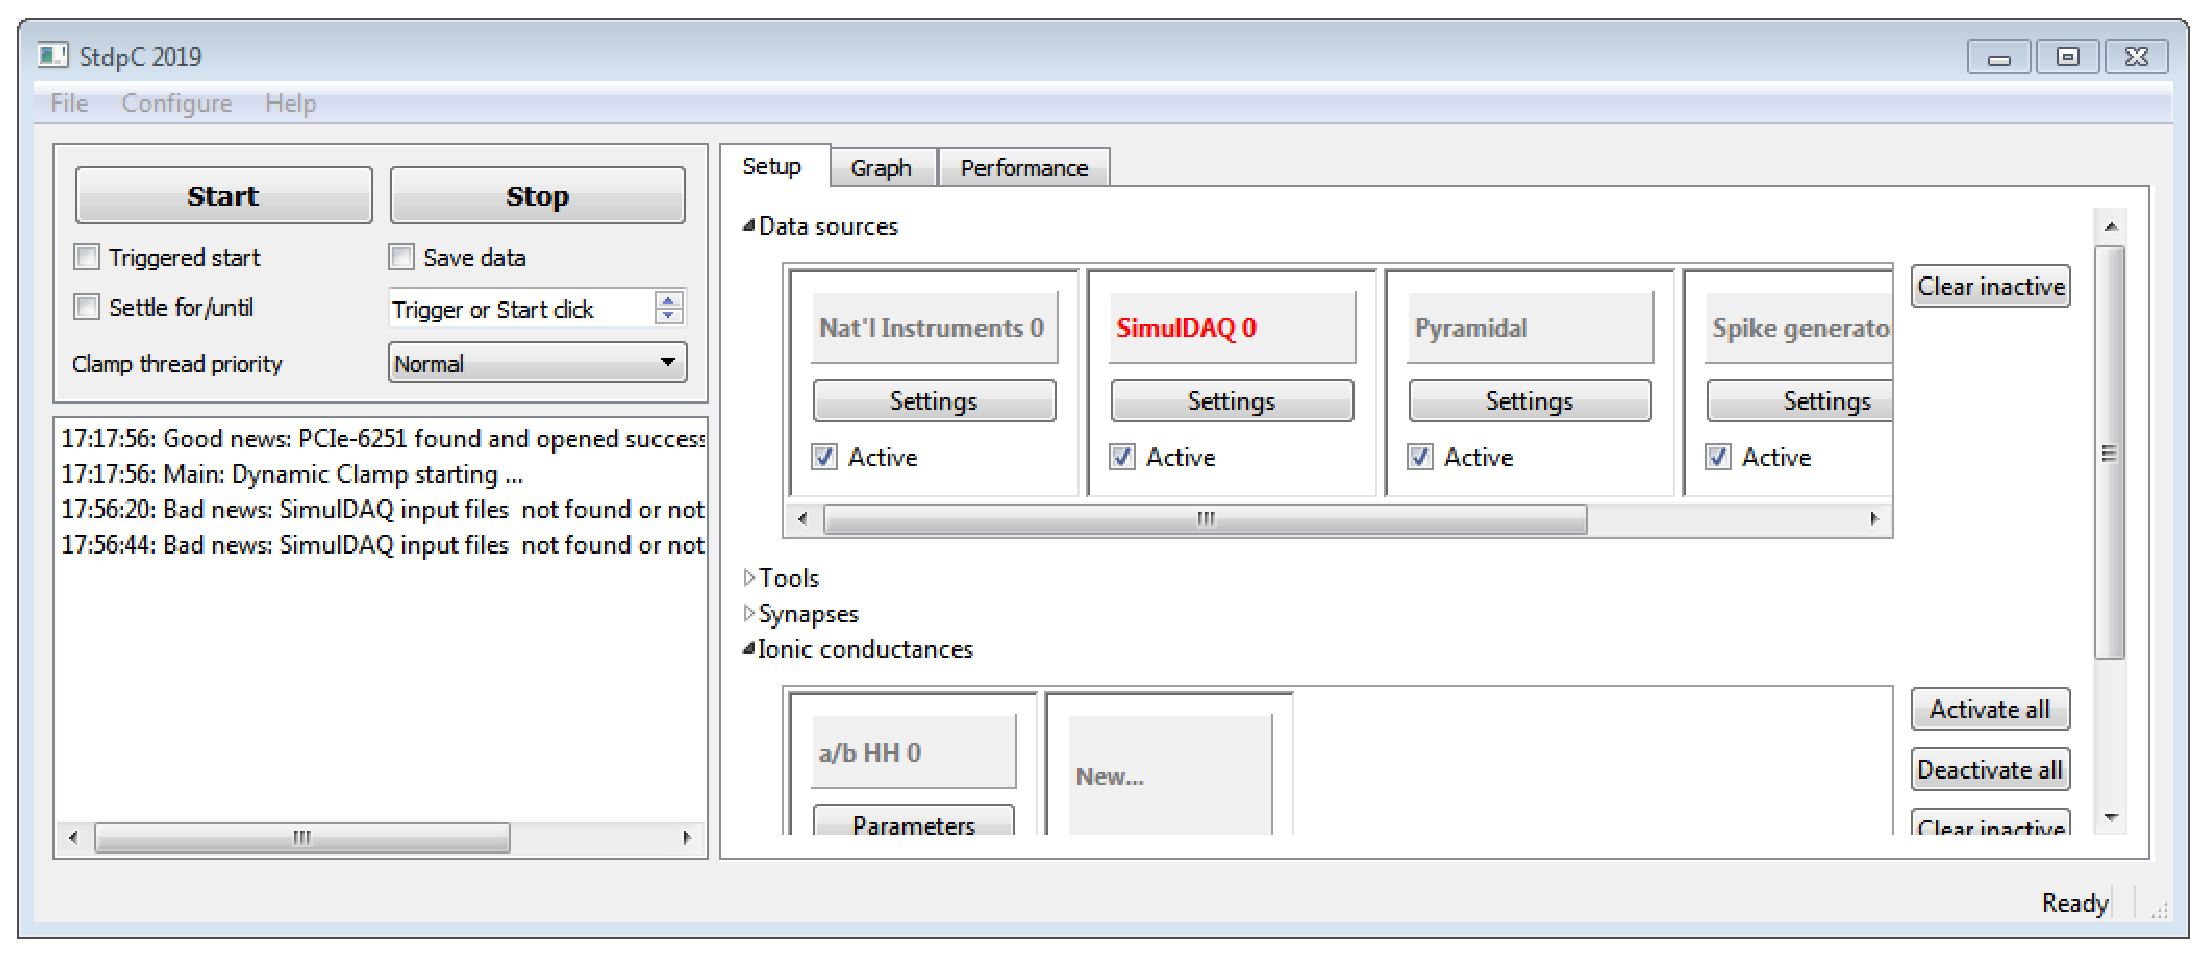
\includegraphics[width=\textwidth]{main}
}
\vspace*{0.5cm}

The main control panel contains different blocks of control for the
different functions of the software -- setting up and configuring acquisition
devices and neuron models (data source control block), adding and configuring
miscellaneous tools (tools block), simulating synapses
(synapse control block), and simulating ionic conductances (Hodgkin-Huxley (HH)
type conductances; conductance control block). The control blocks are front-ends to
more detailed control dialogs. The ``Graph'' and ``Performance'' tabs serve
to display channel and conductance data while the clamp cycle is running, or data
about the clamp cycle performance, respectively. There is a message window in the
left part of the panel that shows system messages. These messages can
be saved for future reference. They are also automatically written to
a local file ``StdpC\_last.log''.


\subsection{Configuration of the Hardware and Control of the Program}
Once StdpC is started, the last known hardware
configuration is loaded (from a local file named
``StdpC.conf''). Other parameters are initialized with default
values that are pre-compiled into the software. The message window
will show a message whether the chosen hardware was successfully
initialized.
Failing hardware initialization can have several causes: \\[-0.2cm]
\begin{myenum}
\item If using the DigiData 1200(A): \\
StdpC's default address for the board is 0x320 (hexadecimal), which
is the default address of the board, but the specific board can have been
configured to use another range of addresses. Possible values are 0x340,
0x360, 0x380, 0x3A0, 0x3C0, etc. Make sure that the correct address is
entered in the ``Digidata'' dialog.
\item If using a National Instruments board: \\
Make sure that NIDAQmx is installed and the board is working properly
(using the NI Automation explorer). Make sure your device is in the
list of devices that support NIDAQmx (as opposed to the older devices
supporting ``old style'' NIDAQ / NIDAQ legacy only).
\item I you are running with simulated data acquisition (SimulDAQ): \\
Make sure that you have a correctly formatted input file for the
membrane potential of cells and that the file name in the ``SimulDAQ''
dialog points to the right location of this file. Also make sure that the
location the output file name points to is writeable to you.
\end{myenum}

\noindent
\parbox{0.45\textwidth}{
	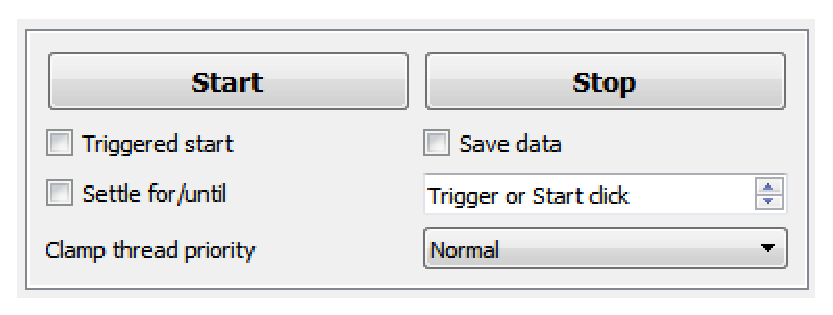
\includegraphics[scale=0.5]{runctrl}
} \hfill
\parbox{0.53\textwidth}{The remaining controls are the ``start'' and the ``stop'' button.  The
``start'' button initiates the start of dynamic clamp cycles. In
particular, pressing this button will stop a running dynamic clamp
thread, load the settings from all dialogs into memory, and
start the dynamic clamp thread again with the new settings. The
dynamic clamp thread will then run until stopped by pressing the
``stop'' button.
} \\

The following additional controls are found in this area:
\begin{myitem}
	\item ``Triggered start'': When checked, pressing ``Start'' will prime the clamp cycle to wait
	until a signal on a digital input channel is received before engaging the cycle. The trigger channel
	is set in the \emph{Start trigger} dialog in the \emph{Configure} menu.
	\item ``Settle for/until:'' When checked, pressing ``Start'' will start the clamp cycle in a reduced
	mode, in which only tools and conductances selected to be active ``when settling'' are enabled.
	The settling period can be specified in seconds or set to 0, meaning indefinite settling. When the 
	settling period is over, ``Start'' is pressed again, or a trigger input is applied, the full clamp
	cycle is immediately engaged.
	\item ``Save data'': Enable or disable data saving, see section \ref{datasaving}.
	\item ``Clamp thread priority'': Set the priority of the thread running the clamp cycle. We recommend
	using the default ``Highest'' priority, as ``Time-critical'' may be unstable and cause freezing.
	Depending on your system, other settings may be preferable, however.
\end{myitem}

The data acquisition hardware can be chosen in the data source control block in the setup tab.
The specific hardware settings can be adjusted in the ``Settings'' dialog of each added device.

Other general control elements can be found in the menus of the main
menu bar. 
\begin{myitem}
\item ``File'' menu:
\
\begin{itemize}
\item[-] ``Load Protocol'': Load parameter settings from a previous
  session. The standard file name extension for these is ``cpr'',
  albeit the settings are saved in plain ASCII format.
\item[-] ``Save Protocol'': Save the current parameter settings into a
  file for later use or documentation.
 \item[-] ``Load Script'': Load a script for experiment
   automation. Scripting is described in section \ref{scriptsect}.
\item[-] ``Unload Script'': Remove a script from memory and use StdpC
  interactively.
\item[-] ``Export Log'': Export the contents of the message box to a
  file.
\item[-] ``Clear Log'': Remove the message box contents.
\item[-] ``Exit'': Quit StdpC.
\end{itemize}
\item ``Config'' menu:
\begin{itemize}
\item['] ``Start trigger'' lets you select a digital input channel from your National Instruments
board for triggered clamp starting.
\item[-] ``Data saving'' Shows a dialog to configure data saving
  settings, see section \ref{datasaving}.
\end{itemize}
\item ``Help'': Offers a brief description about StdpC. 
\end{myitem}


\subsection{Data sources}

\noindent
\parbox{\textwidth}{
	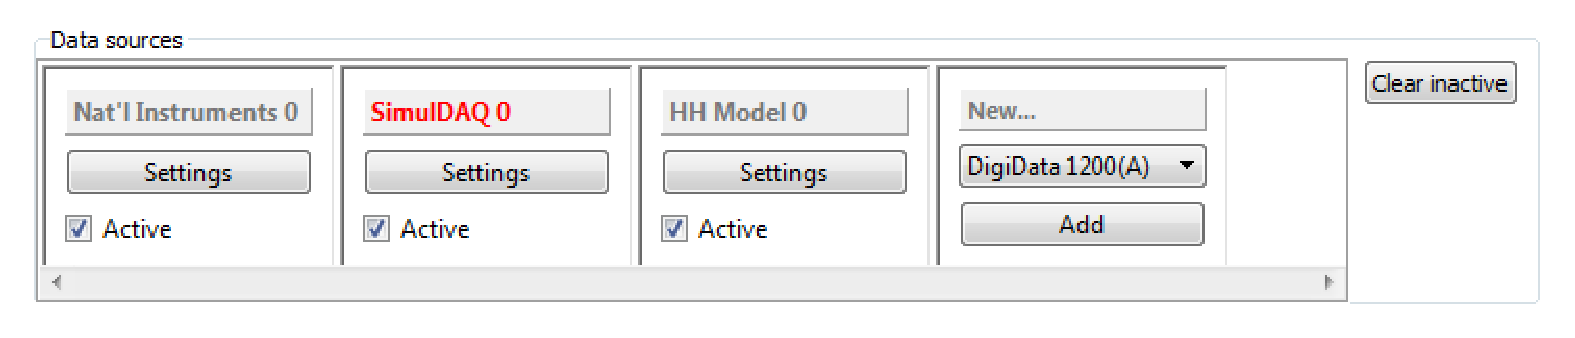
\includegraphics[scale=0.5]{datasources}
} \\[0.2cm]

The data sources control block is used to configure all acquisition devices,
recorded inputs, spike generators and Hodgkin-Huxley models. Sources are added
by selecting the appropriate type in the rightmost box in the list, labelled
``New...'', and clicking ``Add''. An initially inactive data source is then added
to the list, which can be configured by clicking the ``Settings'' button and
activated by checking the ``Active'' checkbox. If the configuration fails, the
failed data source's title will be highlighted in red. When a data source is no
longer required, it can be removed by deactivating it and clicking the
``Clear inactive'' button to the right of the list.

\subsubsection{Digidata 1200(A)}
The Digidata 1200/1200A settings are limited to device address, which is given
in hexadecimal. Channels are configured in subordinate dialogs (see below).
\\
\emph{Scripting:} Script access is given through the \texttt{DigiDatap[\#]} variable.
Only input/output channels are available for scripting, see below.

\subsubsection{National Instruments}
National Instruments devices are configured by giving the exact name of the device,
usually ``Dev1'' or similar. This can be found e.g. by running the NI MAX utility
that comes with the device drivers. Channels are configured in subordinate dialogs (see below).
\\
\emph{Scripting:} Script access is given through the \texttt{NIDAQp[\#]} variable.
Only input/output channels are available for scripting, see below.

\subsubsection{SimulDAQ}
For testing and debugging, you can use a text file with recorded voltages in place of
an acquisition device. Each line corresponds to a set of data points: The first column
gives the time, while subsequent columns (separated by any non-numeric character(s)) give
voltage values. In the SimulDAQ settings dialog, configure the number of input channels
to reflect the data - note that all data are read, and a mismatch between the settings and
the data will most likely result in garbage. SimulDAQ output provides an alternative to
normal data saving. Both input and output channels are configured in subordinate dialogs (see below).
\\
\emph{Scripting:} Script access is given through the \texttt{SDAQp[\#]} variable.
Only input/output channels are available for scripting, see below.

\subsubsection{Input channel configuration} \label{inchnconfig}

The \emph{Input Channels} dialog contains the basic configurable properties
for the input channels, like whether they are going to be active or not,
their acquisition range and conversion factor, along with some more StdpC specific
properties, like whether spike detection is going to be on or
off on them (required for spike-time dependent plasticity rules in synapses), and if it is on, what spike
detection threshold will be applied, and finally whether the channel is
going to be saved or not during dynamic clamping (Section \ref{datasaving}). Always make sure that the
right conversion factor is applied for each active channel, and a
sufficiently wide acquisition range is set in order to prevent out of range
data being cut off of the recorded data. \\
Input channels of an active, fully configured acquisition device can be AEC-calibrated from here by
clicking ``Calibrate''. For more details about AEC and the calibration process, see section \ref{eleccomp}.\\

\noindent
\parbox{\textwidth}{
	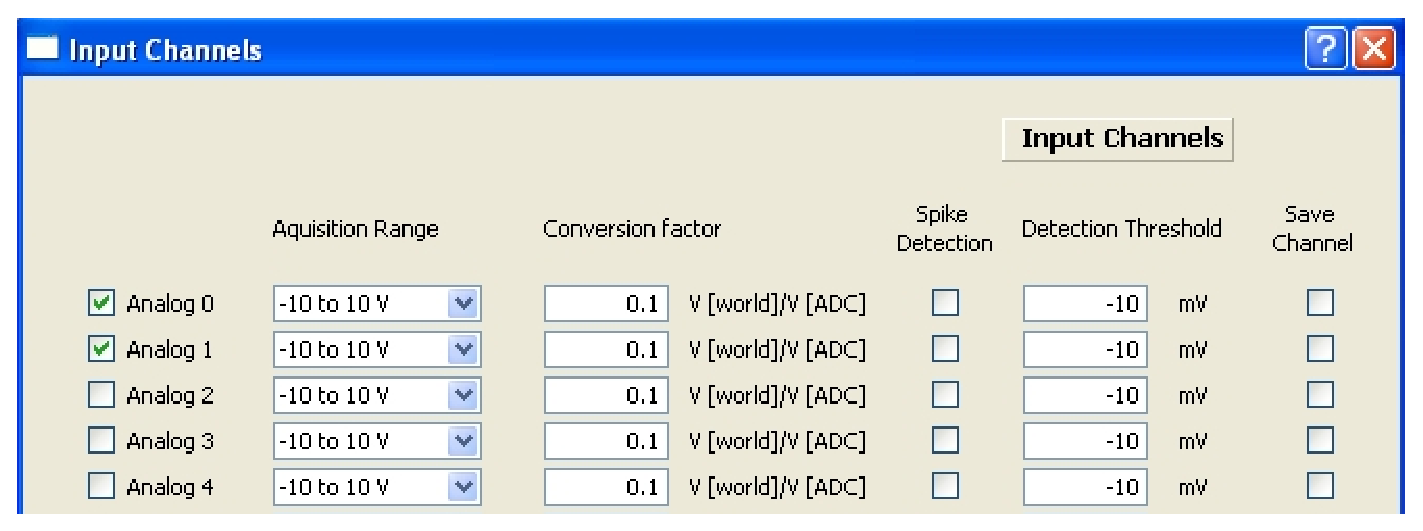
\includegraphics[scale=0.5]{inputChnDialog}
} \\[0.2cm]

\noindent
\emph{Scripting:} Script access to input channels is given through the \texttt{<device>.inChn[\#]} variable
(e.g. \texttt{NIDAQp[0].inChn[0].active}).
The following members are available for scripting: \\
\begin{tabularx}{\linewidth}{|ll|X|}
	\hline
	{\bf \textless{}device\textgreater.inChn[\#].\textvisiblespace} & {\bf Value range} & {\bf Notes} \\
	\hline
	\texttt{active} & 0,1 & Channels must be initially active. Deactivating a channel suspends all
	  synapses and conductances that rely on it. \\
	\texttt{spkDetect} & 0,1 & Spike detection on/off \\
	\texttt{spkDetectThreshold} & double & \\
	\texttt{bias} & double & A constant bias added to every sample \\
	\hline
\end{tabularx}


\subsubsection{Output channel configuration} \label{outchnconfig}

The \emph{Output Channels} dialog contains the basic configurable properties
for the output channels, like whether they are going to be active or not,
their acquisition range and conversion factor, what is the bias current
level applied on that channel if any, and finally whether the channel is
going to be saved or not during dynamic clamping (Section
\ref{datasaving}). Always make sure that the right conversion factor is
applied for each active channel, and a sufficiently wide acquisition range
is set in order to prevent out of range values being cut off of the
injected current.\\

\noindent
\parbox{\textwidth}{
	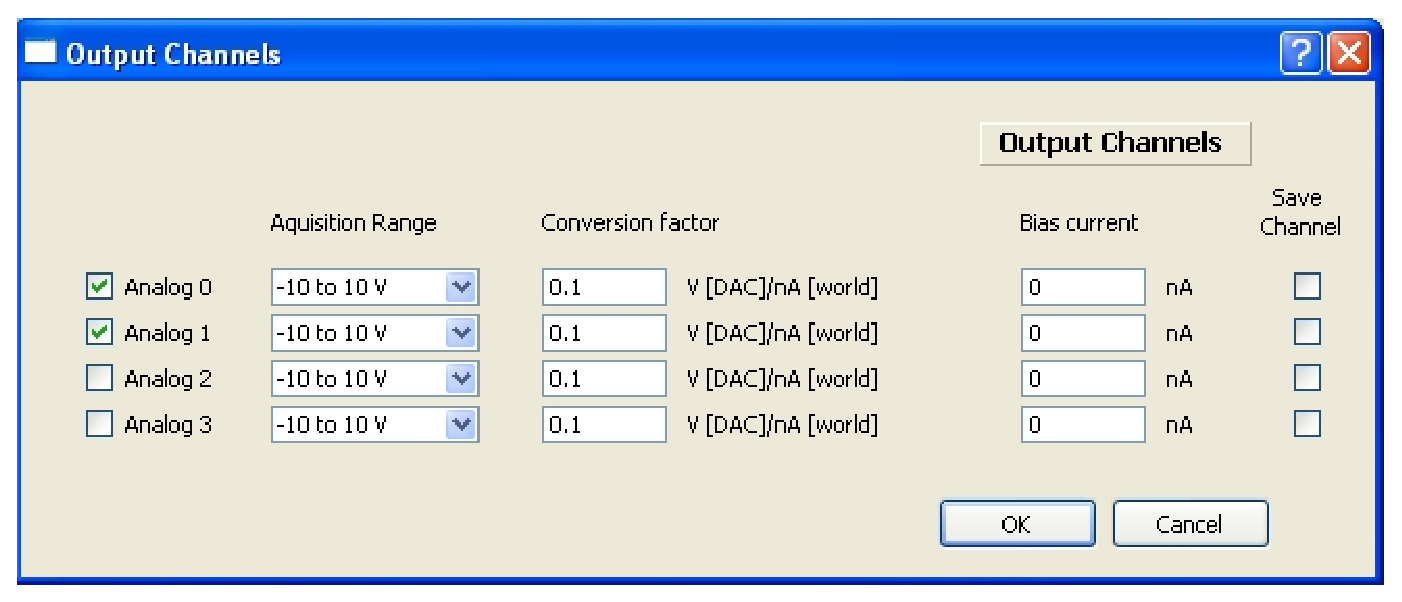
\includegraphics[scale=0.5]{outputChnDialog}
} \\[0.2cm]

\noindent
\emph{Scripting:} Script access to output channels is given through the \texttt{<device>.outChn[\#]} variable
(e.g. \texttt{NIDAQp[0].outChn[0].active}).
The following members are available for scripting: \\
\begin{tabularx}{\linewidth}{|ll|X|}
	\hline
	{\bf \textless{}device\textgreater.outChn[\#].\textvisiblespace} & {\bf Value range} & {\bf Notes} \\
	\hline
	\texttt{active} & 0,1 & Channels must be initially active. Deactivating a channel suspends all
	synapses and conductances that rely on it. \\
	\texttt{bias} & double & Bias current \\
	\hline
\end{tabularx}


\subsubsection{Hodgkin-Huxley model neurons} \label{HHmodels}

This data source type creates a single membrane compartment model.
The base parameters for a model are its capacitance and a passive leak conductance,
defined with its conductivity ``g Leak'' and its reversal potential ``E Leak''.
Below these parameters, there is a list of instances, which can be thought of as
individual neurons. Each instance can be active or inactive, and it creates a voltage
channel (``VChan'', with options for data saving, voltage offset, and spike detection),
and a current channel (``IChan'', with options for data saving and current offset).
These channels appear alongside analog input and output channels, respectively, in
channel selection dialogs elsewhere. Instance-specific channels are labelled ``HH X:Y'',
where X is the model number, and Y is the instance number. \\
In order to complete a neuron model, you will need to define a number of Hodgkin-Huxley
conductances (see section \ref{HHcurrents}) and assign these to the model. This is done
by selecting the model's ``All'' channel (``HH X:all'') for both the voltage and the current channel
assignment of the conductance. Using the ``All'' channel guarantees that the conductance
is applied to all active instances of the model. \\
In a similar manner, synapses can be assigned to all active instances of a model
using the ``All'' channel, or to a specific instance using that instance's numbered
channel.\\

\noindent
\parbox{\textwidth}{
	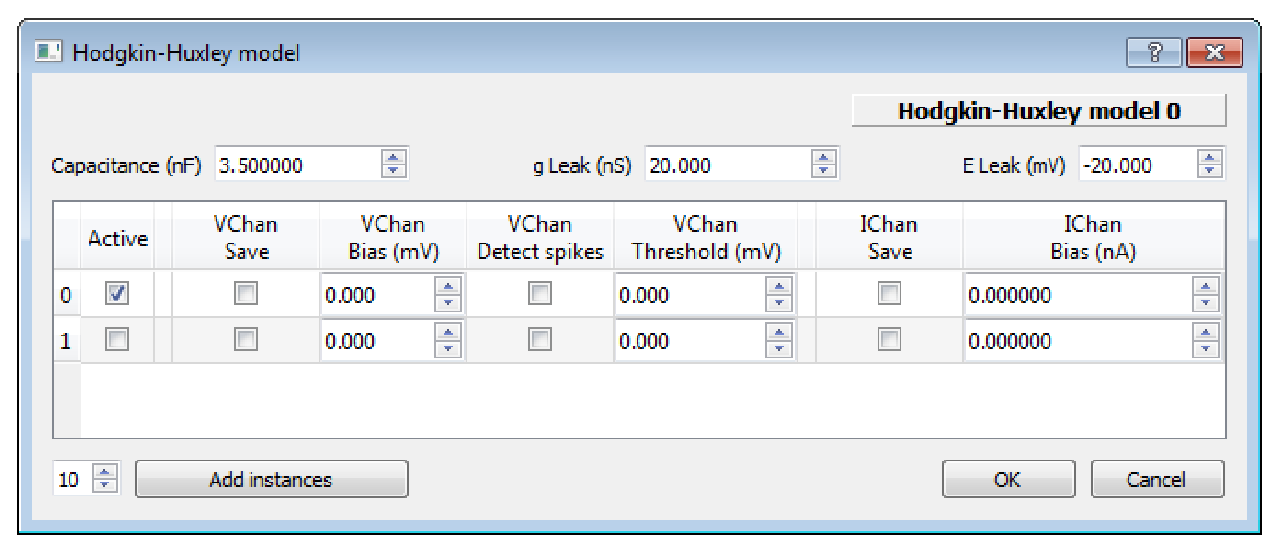
\includegraphics[scale=0.5]{HHmodel}
} \\[0.2cm]

\noindent
\emph{Scripting:} Script access to models is given through the \texttt{HHNeuronp[\#]} variable.
The following members are available for scripting: \\
\begin{tabularx}{\linewidth}{|ll|X|}
	\hline
	{\bf HHNeuronp[\#].\textvisiblespace} & {\bf Value range} & {\bf Notes} \\
	\hline
	\texttt{active} & 0,1 & Models must be initially active. Deactivating a model suspends all of
	its instances. \\
	\texttt{C} & double & \\
	\texttt{gLeak} & double & \\
	\texttt{ELeak} & double & \\
	\texttt{inst[\#].active} & 0,1 & Model instances must be initially active. Deactivating a model instance
	suspends its input and output channels and all synapses and conductances that rely on them. \\
	\texttt{inst[\#].inChn.spkDetect} & 0,1 & Spike detection on/off \\
	\texttt{inst[\#].inChn.spkDetectThreshold} & double & \\
	\texttt{inst[\#].inChn.bias} & double & Bias voltage \\
	\texttt{inst[\#].outChn.bias} & double & Bias current \\
	\hline
\end{tabularx}

\subsubsection{Spike generator} \label{spikegen}
The spike generator unit can replace a presynaptic cell. It generates spikes of a 
predefined shape, in a temporal pattern defined by the user. It can operate in
a triggered mode, producing spike patterns (bursts) in response to a threshold crossing
on a different (measured) channel, or in stand-alone mode, producing bursts in
periodic fashion. \\
Note: In earlier versions of StdpC, the spike generator could also be used to
replay recorded voltages from files. This function is no longer available
here, but can easily be replaced by using a SimulDAQ data source instead.\\

\noindent
\parbox{\textwidth}{
	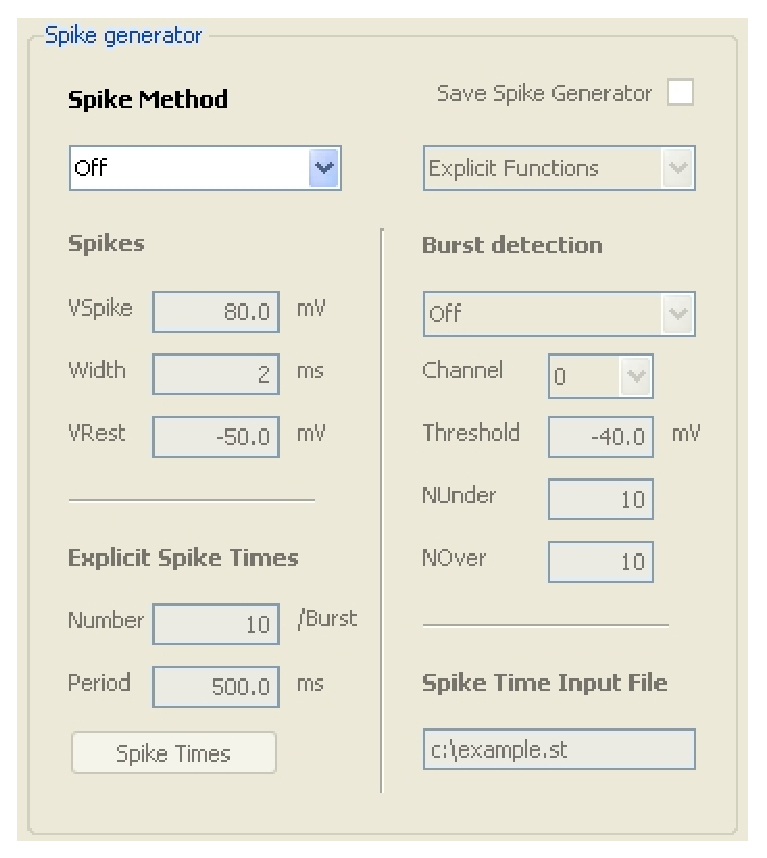
\includegraphics[scale=0.5]{spikeGenBlock}
} \\[0.2cm]

The control elements for the spike generator are: \\

``Spikes'' : Each spike rises exponentially from the resting potential, reaches its peak
at the designated spike time, then drops off symmetrically to its rise.
\begin{myitem}
	\item VSpike: The amplitude of the spikes generated
	\item Width: The width of spikes in ms
	\item VRest: The resting potential from which the spikes depart
\end{myitem}

``Burst detection''
\begin{myitem}
	\item The transition combo allows to choose whether to trigger bursts
	independently of external events (Off), or whether to trigger an
	event for low to high or high to low transitions through a threshold
	value. Threshold detection is performed on a separate channel for each
	instance of the spike generator, see below.
	\item Threshold: For low$\rightarrow$high detection, an event
	is triggered whenever tUnder milliseconds were below threshold and
	afterwards tOver milliseconds were above. Note that for noisy
	signals it may be  necessary to increase both numbers for reliable
	detection.
	\item When the respective ``Contiguous'' box is checked, the events
	below and above are required to be contiguous. Otherwise, time spent
	below or above threshold is added up cumulatively.
	\item Strictly contiguous: Checking this box means that an event is
	triggered if and only if the burst detection voltage makes a single,
	smooth threshold crossing.
\end{myitem}

``Instances''
\begin{myitem}
	\item The spike generator can be instantiated multiple times. Each instance
	has options to save the output, to offset it by a fixed value, and to detect
	threshold crossings on a specific channel, at a given threshold voltage.
	\item Each spike generator instance creates a voltage channel named ``SG X:Y'',
	where X is the spike generator number, and Y is the instance number.
\end{myitem}

``Spike times''
\begin{myitem}
	\item Loop burst sequence: If this box is checked, the burst sequence is repeated.
	Otherwise, the spike generator will turn itself off once all bursts are generated.
	\item Period: If burst detection is turned off, each burst is generated in order,
	triggered at the start of the clamp cycle, and once for each period. Bursts that last
	longer than the period are truncated.
	\item Spike times are given in the table at the bottom of the dialog. Each line
	corresponds to one burst, which has an unrestricted number of spikes. Spike times
	are given in milliseconds relative to the start of the burst. Note: Spike times
	are sorted in ascending order when the dialog is closed and before saving to file.
	Spike times at t=0.0 are ignored.
	\item Load, Save buttons: Burst patterns can be read from and written to files.
	StdpC expects descriptions of spike patterns containing 
	\begin{myitem}
		\item[-] An integer denoting the number of spikes in the pattern
		\item[-] A matching number of spike times in seconds, measured from the
		detection event. 
	\end{myitem}
	These pattern descriptions are best separated by newlines. Note: Previous versions
	of StdpC allowed input files with a single spike sequence in untriggered mode. Since
	all modes now allow several bursts, such files must be converted; simply add the number
	of spikes before the first spike time value.
\end{myitem}

\noindent
\emph{Scripting:} Script access to spike generators is given through the \texttt{SGp[\#]} variable.
The following members are available for scripting: \\
\begin{tabularx}{\linewidth}{|ll|X|}
	\hline
	{\bf SGp[\#].\textvisiblespace} & {\bf Value range} & {\bf Notes} \\
	\hline
	\texttt{active} & 0,1 & Spike generators must be initially active. Deactivating a spike generator
	suspends all of	its instances. \\
	\texttt{VSpike} & double & \\
	\texttt{spkTimeScaling} & double & = 5000 / Spike width (ms)\\
	\texttt{VRest} & double & \\
	\texttt{bdType} & 0,1,2 & Burst detection: 0-off, 1-low to high, 2-high to low \\
	\texttt{bdtUnder} & double & \\
	\texttt{bdtUnderCont} & 0,1 & Contiguous on/off \\
	\texttt{bdtOver} & double & \\
	\texttt{bdtOverCont} & double & \\
	\texttt{bdStrictlyCont} & double & \\
	\texttt{period} & double & \\
	\texttt{loopBursts} & double & \\
	\texttt{SpikeT[\#][\#]} & double & Spike times in s relative to burst initiation.
	 The first index is for the burst, the second for the spike. Indexing is zero-based.
	 Note that if bursts or spikes are added by a script, they will exist from the moment the clamp
	 cycle is started. E.g., if the protocol specifies one burst, and the script defines SpikeT[2][5]
	 at any time,
	 there will be one empty burst (index 1) and one burst with 6 spikes at time 0 (index 2). Empty
	 bursts are not skipped, they just happen to produce no spikes. Spike times at or below 0 are ignored. \\
	\texttt{inst[\#].active} & 0,1 & Spike generator instances must be initially active.
	 Deactivating an instance suspends its voltage channel and all synapses and conductances that rely on it. \\
	\texttt{inst[\#].inChn.bias} & double & Bias voltage \\
	\texttt{inst[\#].bdThresh} & double & Burst detection threshold \\
	\hline
\end{tabularx}

\subsubsection{Voltage stepper}
The voltage stepper generates a series of square voltage pulses that can be used e.g. for
software-defined voltage clamp protocols.

\noindent
\parbox{0.28\textwidth}{
	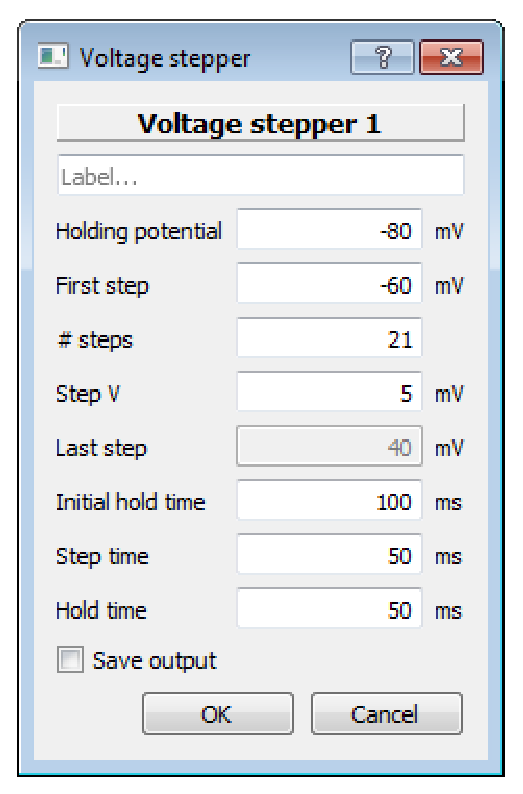
\includegraphics[scale=0.5]{VoltageStepper}
}
\hfill
\parbox{0.7\textwidth}{
	The following parameters control the step generation process:
	\begin{myitem}
		\item Holding potential: The base voltage before, between, and after any steps.
		\item First step: The voltage of the first step.
		\item \# steps: The number of steps to be generated.
		\item Step V: The voltage offset added to each step after the first. E.g., with a first step
		at -60 mV and a step V of 5 mV, the second step will be at -55 mV, the third at -50 mV, etc.
		\item Last step: Displays the voltage of the final step in the series, given the three inputs
		above.
		\item Initial hold time: Duration of the period before the first step, during with the holding
		potential is applied.
	\end{myitem}
}
\begin{myitem}
	\item Step time: Duration of each step.
	\item Hold time: Duration of the holding period between steps.
	\item Save output: Saves the channel data to file, if data saving is activated.
\end{myitem}
The voltage stepper module does not currently have any scriptable variables.


\subsection{Synapses}

\noindent
\parbox{\textwidth}{
	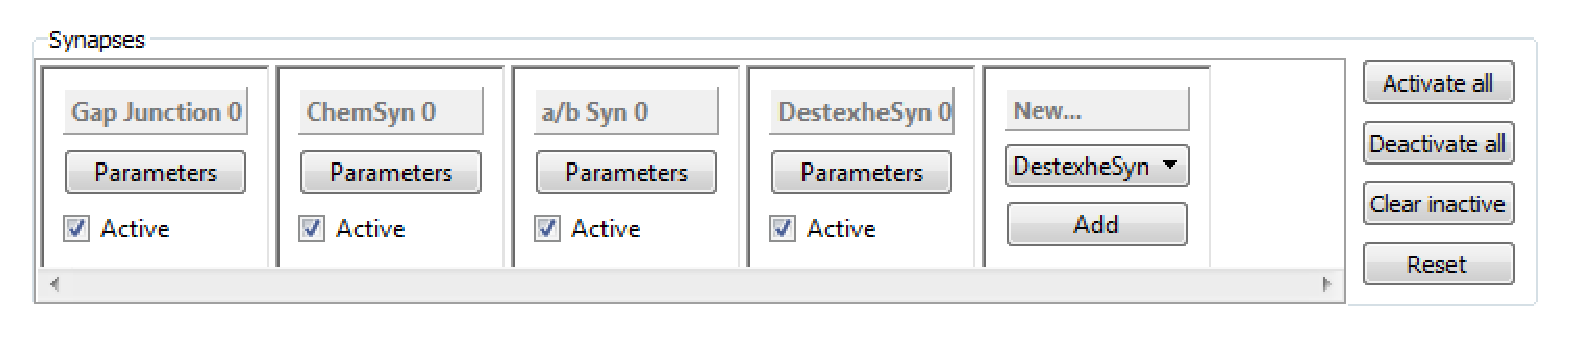
\includegraphics[scale=0.5]{synapseBlock}
} \\[0.2cm]

The synapse control block contains an arbitrary number of synapse configurations.
Synapses are added by selecting the appropriate type in the rightmost box in the
list, labelled ``New...'', and clicking ``Add''. An initially active synapse is
then added to the list, which can be configured by clicking the ``Parameters'' button and
activated or deactivated by checking or unchecking the ``Active'' checkbox. When a synapse is no
longer required, it can be removed by deactivating it and clicking the
``Clear inactive'' button to the right of the list. The ``Reset'' button just below that
resets the entire control block to its most recent saved state, i.e. the state it was in upon
program start, loading or saving a protocol, or clicking the ``Start'' button.

\subsubsection{Electrical synapses (Gap Junctions)}

\noindent
\parbox{0.4\textwidth}{
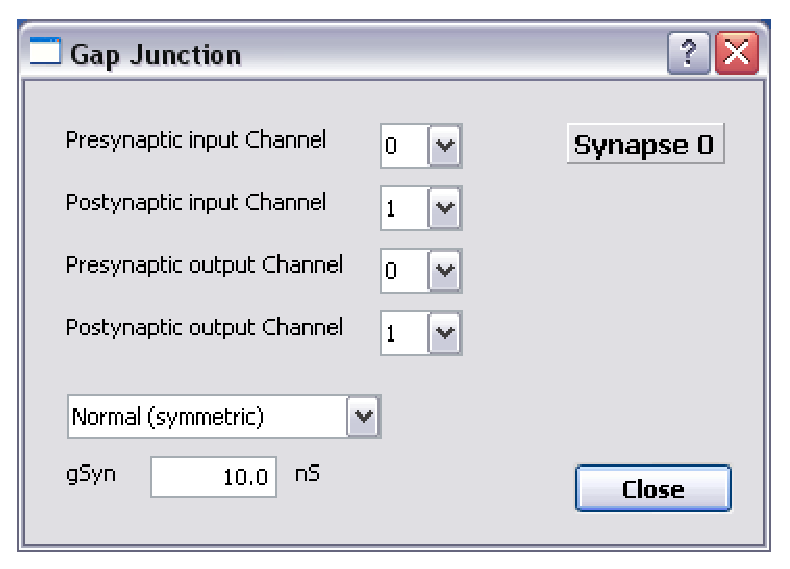
\includegraphics[scale=0.4]{gapJunctionDialog}
}
\hfill
\parbox{0.48\textwidth}{
The currents $I_{\text{pre}}$ and $I_{\text{post}}$ to be injected
into the pre- and post-synaptic cells, respectively, are calculated
according to:
\begin{align}
  I_{\text{post}}(t) &= g_{\text{Syn}} [V_{\text{pre}}(t) - V_{\text{post}}(t)],  \\
  \text{and} \quad I_{\text{pre}}(t) &= -I_{\text{post}}(t), 
\end{align}
where $V_{\text{pre}}(t)$ and $V_{\text{post}}(t)$ are the membrane
potential of the two cells. If the gap junction is chosen as
rectifying, $I_x (t)= 0$ if $V_{\text{pre}}(t) < V_{\text{post}}(t)$.
} \\[0.2cm]
The controls in the gap junction dialog are
\begin{myitem}
	\item Channel assignments: Each individual gap junction is assigned to presynaptic
	and postsynaptic voltage (input) and current (output) channels and can be individually
	turned on and off. \\
	Note that assignments to neuron model ``All'' channels are resolved intelligently
	(e.g. assigning presynaptic V and I to HH 0:All and postsynaptic V and I to analog channels
	gives rise to one synapse per active model instance)
	and on an all-to-all basis (e.g. assigning presynaptic V and I to HH 0:All and 
	postsynaptic V and I to HH 1:All causes every instance of HH 0 to form synapses with
	each instance of HH 1).
	\item Rectification: You can choose whether the gap junction is ordinary (``Normal (symmetric)'', the
	current can flow from the pre-synaptic cell to the postsynaptic cell
	and vice versa; both cells have perfectly symmetrical roles in this
	case) or rectifying (positive current can only flow from the presynaptic
	cell to the postsynaptic cell but not in the other direction).
	\item gSyn: The synaptic conductance in nS.
\end{myitem}

\noindent
\emph{Scripting:} Script access to gap junctions is given through the \texttt{ESynp[\#]} variable.
The following members are available for scripting: \\
\begin{tabularx}{\linewidth}{|ll|X|}
	\hline
	{\bf ESynp[\#].\textvisiblespace} & {\bf Value range} & {\bf Notes} \\
	\hline
	\texttt{active} & 0,1 & Synapses must be initially active. Deactivating a synapse suspends all
	its assignments. \\
	\texttt{assign[\#].active} & 0,1 & Assignments must be initially active. \\
	\texttt{type} & 0,1 & 0-normal, 1-rectifying \\
	\texttt{gSyn} & double & \\
	\hline
\end{tabularx}


\subsubsection{Chemical Synapses}
The current to be
injected into the postsynaptic cell, $I_{\text{post}}$, is calculated
in each dynamic clamp cycle using a first order kinetics model of the
release of neurotransmitter, an additional
inactivation term, $h(t)$, to simulate short term depression, and
an optional magnesium block term, $g_{\text{Mg}}(t)$:
\begin{align}
  I_{\text{post}} = g_{\text{Syn}} \, g_{\text{Mg}}(t) \, S(t) \, h(t) [V_{\text{Syn}} -
    V_{\text{post}}(t)],
\end{align}
where the instantaneous activation, S(t), and inactivation, h(t), terms are
given by the differential equations
\begin{align}
(1-S_\infty(V_{\text{pre}})) \tau_{\text{Syn}} \frac{dS(t)}{dt} &=
(S_\infty(V_{\text{pre}}) - S(t)) \\ \tau_h \frac{dh(t)}{dt} &=
h_\infty(V_{\text{pre}}) - h(t),
\end{align}
where
\begin{align}
S_\infty(V_{\text{pre}}) &= \left\{
\begin{array}{ll}
  \tanh\left[\frac{V_x(t) - V_{\text{Thresh}}}{V_{\text{Slope}}}
    \right] & \text{if } V_{\text{pre}} > V_{\text{Thresh}} \\ 0 &
  \text{otherwise}
  \end{array}
\right. \\ 
%
h_\infty(V_{\text{pre}})&=
\frac{A}{1+\exp\left(\frac{V_{\text{pre}} -
    V_{\text{Thresh}}}{V_{\text{Slope}}}\right)}, \\  
\tau_h(V_{\text{pre}})&= \tau_{0} -
\frac{A_\tau}{1+\exp\left(\frac{V_{\text{pre}} -
    V_{\text{Thresh},\tau}}{V_{\text{Slope},\tau}} \right)}
\end{align}
and the optional magnesium block term is given by
\begin{align}
g_{\text{Mg}}(t) &= \frac{1}{1 + F_{\text{Mg}} \, \exp(X_{\text{Mg}} \, V_{\text{post}}(t))}
\end{align}

  The controls in the parameter dialog for the chemical synapse are
  \begin{myitem}
  \item Channel assignments: Each individual synapse is assigned to a presynaptic input channel
  (Presyn V) and postsynaptic input and output channels (Postsyn V, I).
  \item Delay: Each assignment comes with a fixed delay (in ms), which can be used to mimic
  conduction latencies.
\end{myitem}
``General'':
\begin{myitem}
  \item gSyn: The maximal conductance $g_{\text{syn}}$ of the synapse in nS. 
  \item VSyn: The reversal potential $V_{\text{Syn}}$ in mV. 
\item tauSyn: The characteristic time constant $\tau_{\text{Syn}}$ of
  the synapse in ms.  
\item VThresh: The threshold  potential $V_{\text{Thresh}}$ for the
  release of neurotransmitter in mV.  
\item VSlope: The ``slope'' parameter $V_{\text{Slope}}$ of the
  activation curve in mV.  
  \end{myitem}
``Stochastic'':
\begin{myitem}
	\item Check to enable stochastic postsynaptic potentials, defined after \cite{redman1990quantal}.
	Each upward threshold crossing triggers one independently calculated synaptic event, as follows: \\
	The number of active release sites $n$ during a given synaptic event is drawn from a binomial
	distribution, $n \sim B(n_{\text{rel}}, p_{\text{rel}})$. Then, a quantal amplitude factor $q$
	is drawn from a normal distribution, $q \sim N(n, \frac{n \sigma_q}{n_{\text{rel}} p_{\text{rel}}})$,
	and multiplied with $S(t)$ to yield a stochastically scaled postsynaptic conductance.\\ Note, this
	formulation implies that  $g_{\text{syn}}$ is the mean conductance per release site.
	\item \# release sites: Number of independent transmitter release sites $n_{\text{rel}}$.
	\item p(release): Transmitter release probability per site $p_{\text{rel}}$.
	\item PSP variance: The variance $\sigma_q^2$ of the conductance evoked by a single release event.
\end{myitem}
``Fix Vpost'':
\begin{myitem}
	\item Check to draw $V_{\text{post}}$ from a set value, rather than from the
	postsynaptic voltage channel.
	\item Vpost: The fixed value to use for $V_{\text{post}}$.
\end{myitem}
``Mg Block'':
\begin{myitem}
	\item Check to enable the magnesium block term $g_{\text{Mg}}$, defined
	after \cite{FellousSejnowski2003}.
	\item Mg factor: The scaled magnesium concentration $F_{\text{Mg}}$, a unitless value.
	\item Mg exponent: The exponential factor $X_{\text{Mg}}$ in 1/V.
\end{myitem}
``Method'': Any sigmoid, tanh and exponential functions can optionally be computed using
lookup tables. This is less precise than direct methods, but may increase speed
on old computers.

\noindent
\parbox[b]{0.53\textwidth}{
  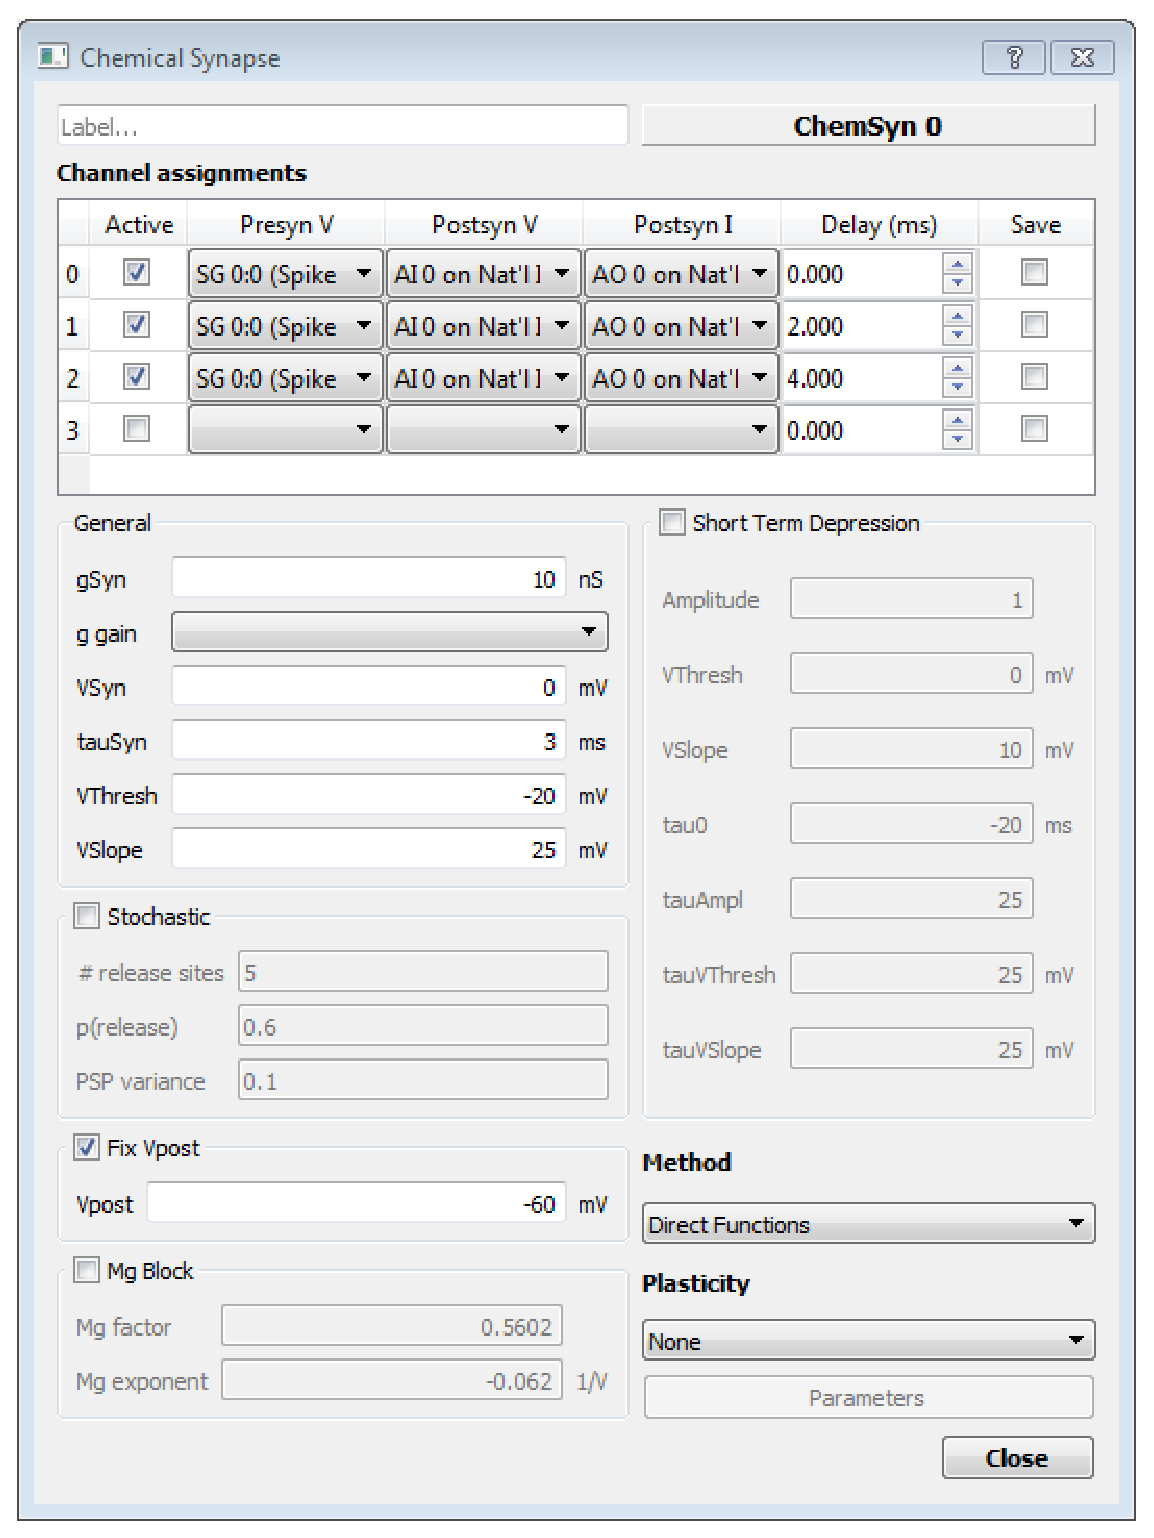
\includegraphics[scale=0.4]{chemicalDialog}
}
\hfill
\parbox[b]{0.5\textwidth}{
``Short Term Depression'':
\begin{myitem}
\item Check to enable.
\item Amplitude: The amplitude of the $h(t)$ depression
  variable. Typically set to 1 (so that $h$ varies between $0$ and
  $1$). This was previously used to switch short term depression on or
  off and remains for historical reasons.
\item VThresh: The threshold potential $V_{\text{Thresh},\tau}$ for
  the activation of $h$ in mV.  
\item VSlope: The ``slope'' parameter of the depression activation
  curve in mV. 
\item tau0, tauAmpl, tauVThresh, and tauVSlope: Parameters $\tau_0$,
  $A_\tau$, $V_{\text{Thresh},\tau}$ and $V_{\text{Slope},\tau}$ for
  the voltage-dependent characteristic time $\tau_h$ of short term depression.
\item The plasticity combo box allows you to choose whether the synapse is
  subject to long term plasticity and according to which model the
  plasticity is determined.\end{myitem}
} \\[0.2cm]
%
For ``Spike STDP'' a spike-timing based
  rule is applied according to the parameters defined in the
  corresponding control panel that appears upon clicking the
  ``Parameters'' button.
  If ``ODE STDP'' is chosen, the synaptic
  plasticity is implemented according to the ordinary differential
  equation (ODE) description in \cite{Abarbanel2002}. Parameters again
  are adjusted in the separate panel that appears after pressing
  ``Parameters''. For details on both methods, see section \ref{STDP}.\\

\noindent
\emph{Scripting:} Script access to chemical synapses is given through the \texttt{CSynp[\#]} variable.
The following members are available for scripting: \\
\begin{tabularx}{\linewidth}{|ll|X|}
	\hline
	{\bf CSynp[\#].\textvisiblespace} & {\bf Value range} & {\bf Notes} \\
	\hline
	\texttt{active} & 0,1 & Synapses must be initially active. Deactivating a synapse suspends all
	its assignments. \\
	\texttt{assign[\#].active} & 0,1 & Assignments must be initially active. \\
	\texttt{gSyn} & double & \\
	\texttt{VSyn} & double & \\
	\texttt{tauSyn} & double & \\
	\texttt{VThresh} & double & \\
	\texttt{VSlope} & double & \\
	\texttt{stochastic} & 0,1 & Stochasticity on/off \\
	\texttt{stoch\_nRel} & int & \\
	\texttt{stoch\_pRel} & double & \\
	\texttt{stoch\_variance} & double & \\
	\texttt{fixVpost} & 0,1 & \\
	\texttt{Vpost} & double & \\
	\texttt{STD} & 0,1 & Short-term depression on/off \\
	\texttt{STDAmpl} & double & \\
	\texttt{STDVThresh} & double & \\
	\texttt{STDVSlope} & double & \\
	\texttt{STDtau0} & double & \\
	\texttt{STDtauAmpl} & double & \\
	\texttt{STDtauVTresh} & double & \\
	\texttt{STDtauVSlope} & double & \\
	\texttt{MgBlock} & 0,1 & \\
	\texttt{MgFac} & double & \\
	\texttt{MgExpo} & double & \\
	\texttt{Plasticity} & 0,1,2 & 0-off, 1-Spike 2-ODE. See below for STDP scripting.\\
	\hline
\end{tabularx}


\subsubsection{Alpha beta synapse}
The $\alpha\beta$ synapse implemented in StdpC is a variation on the
classic Rall synapse \cite{Rall1967} with a pre-synaptic release variable $R$ and a
post-synaptic binding variable $S$ which then gates the synaptic
current. The model is described by:
\begin{align}
I_{\text{syn}}&= g_{\text{syn}} S (V_{\text{rev}} -
V_{\text{post}}) \\
 \frac{dS}{dt} &= \alpha_S (1-S)R - \beta_S S  \\
 \frac{dR}{dt} &= \alpha_R (1-R) \frac{1}{1+
   \exp (\frac{V_{\text{pre}}-V_{\alpha R}}{s_{\alpha R}})} -
 \beta_R R  
\end{align}
\parbox[b]{0.58\textwidth}{
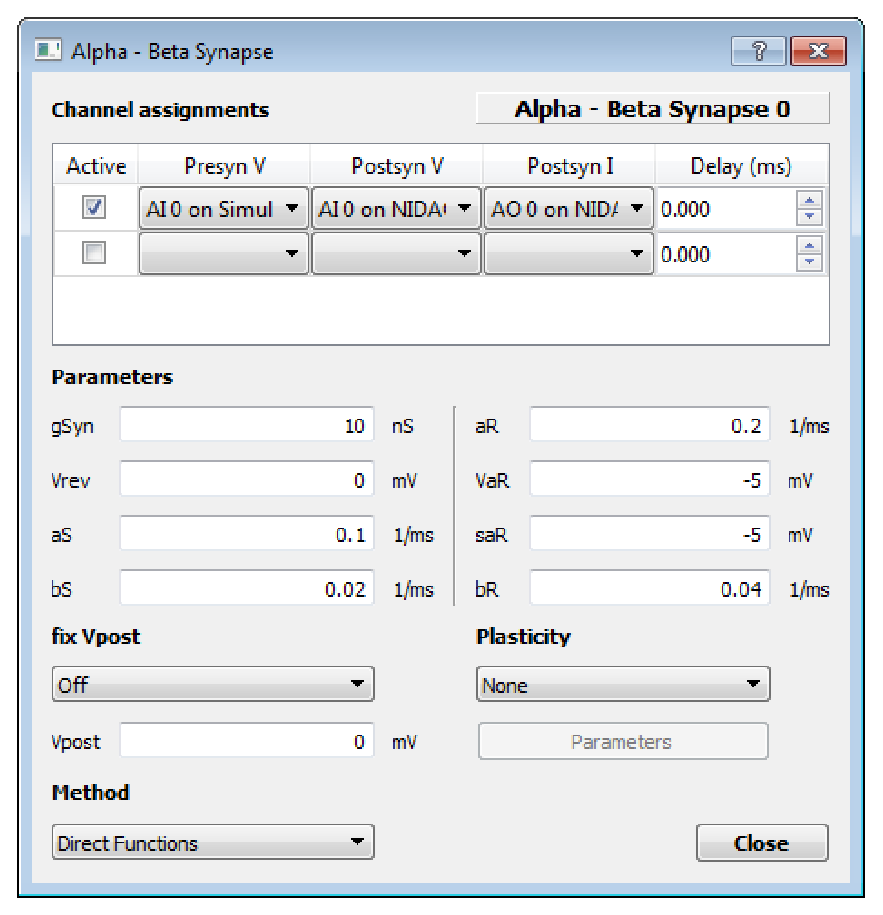
\includegraphics[scale=0.5]{abSynDialog}\\}
\hfill
\parbox[b]{0.4\textwidth}{
\begin{itemize}
\item Channel assignments, method, fixed Vpost and plasticity are described above.
\item gSyn: Maximal synaptic conductance
\item Vrev: Reversal potential of the synapse
\item aS: Rate of transmitter binding to post-synaptic targets
\item bS: Rate of transmitter removal (channel closing)
  postsynaptically
\item aR: Rate of transmitter release when pre-synaptic potential is
  elevated
\end{itemize}
}
\begin{itemize}
	\item VaR: Midpoint of the sigmoid function expressing the level of
	pre-synaptic release as a function of pre-synaptic membrane
	potential
	\item saR: Width of the release sigmoid function
	\item bR: Fall rate of the presynaptic release
\end{itemize}

\noindent
\emph{Scripting:} Script access to alpha-beta synapses is given through the \texttt{abSynp[\#]} variable.
The following members are available for scripting: \\
\begin{tabularx}{\linewidth}{|ll|X|}
	\hline
	{\bf abSynp[\#].\textvisiblespace} & {\bf Value range} & {\bf Notes} \\
	\hline
	\texttt{active} & 0,1 & Synapses must be initially active. Deactivating a synapse suspends all
	its assignments. \\
	\texttt{assign[\#].active} & 0,1 & Assignments must be initially active. \\
	\texttt{gSyn} & double & \\
	\texttt{Vrev} & double & \\
	\texttt{aS} & double & \\
	\texttt{bS} & double & \\
	\texttt{aR} & double & \\
	\texttt{VaR} & double & \\
	\texttt{saR} & double & \\
	\texttt{bR} & double & \\
	\texttt{fixVpost} & 0,1 & \\
	\texttt{Vpost} & double & \\
	\texttt{Plasticity} & 0,1,2 & 0-off, 1-Spike, 2-ODE. See below for STDP scripting. \\
	\hline
\end{tabularx}


\subsubsection{Destexhe synapse}
This synapse model is the simple first order synapse description
introduced in \cite{Destexhe1994}. In brief,
\begin{align}
I_{\text{syn}}&= g_{\text{syn}} S (V_{\text{rev}} -
V_{\text{post}}) \\
\frac{dS}{dt} &= \left\{ \begin{array}{ll} 
  \alpha (1-S) - \beta S & \text{if } t-t_{\text{spike}} < t_{\text{release}} \\
- \beta S & \text{otherwise} 
\end{array} \right.
\end{align}
where $t_{\text{spike}}$ is the time of the occurrence of the last
spike in the pre-synaptic neuron.

\noindent
\parbox[b]{0.58\textwidth}{
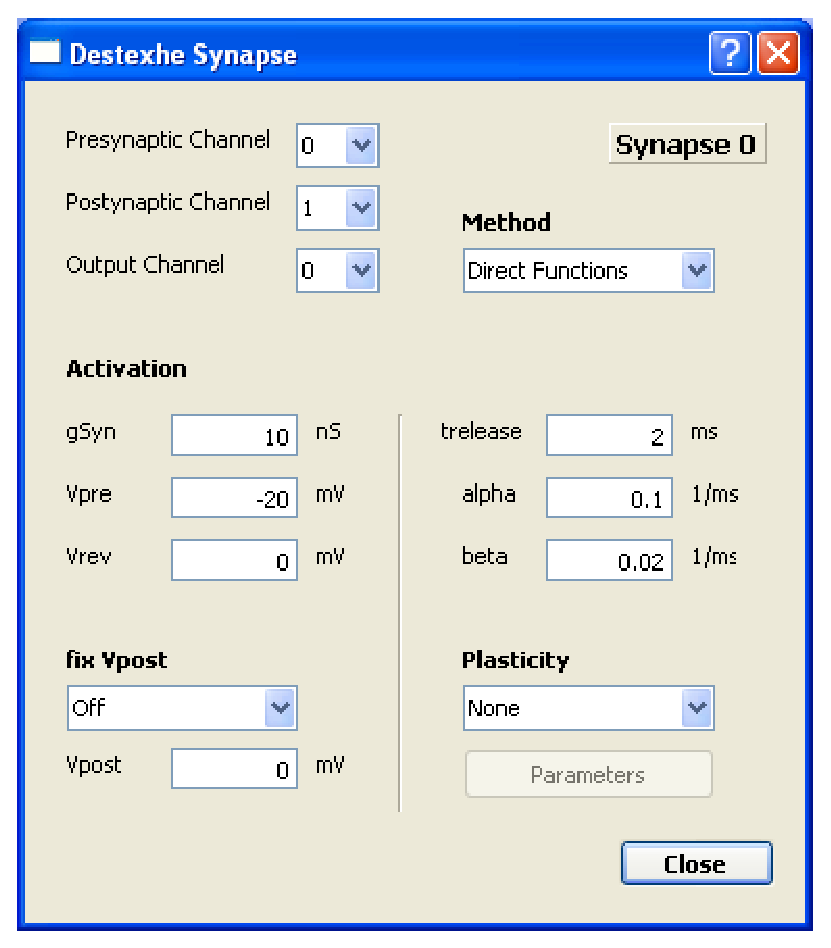
\includegraphics[scale=0.5]{destexheSynDialog}}
\hfill
\parbox[b]{0.4\textwidth}{
\begin{itemize}
\item Channel assignments, method, fixed Vpost and plasticity are described above.
\item gSyn: Maximal synaptic conductance
\item Vpre: pre-synaptic threshold for triggering synaptic transmitter
  release
\item Vrev: Reversal potential of the synapse
\item trelease: The time (duration) of transmitter release after a
  presynaptic spike
\item alpha: The rise rate for the EPSCs
\item beta: the fall (decay) rate for the EPSCs
\end{itemize}
}\\

\noindent
\emph{Scripting:} Script access to Destexhe synapses is given through the \texttt{DxheSynp[\#]} variable.
The following members are available for scripting: \\
\begin{tabularx}{\linewidth}{|ll|X|}
	\hline
	{\bf abSynp[\#].\textvisiblespace} & {\bf Value range} & {\bf Notes} \\
	\hline
	\texttt{active} & 0,1 & Synapses must be initially active. Deactivating a synapse suspends all
	its assignments. \\
	\texttt{assign[\#].active} & 0,1 & Assignments must be initially active. \\
	\texttt{gSyn} & double & \\
	\texttt{Vpre} & double & \\
	\texttt{Vrev} & double & \\
	\texttt{trelease} & double & \\
	\texttt{alpha} & double & \\
	\texttt{beta} & double & \\
	\texttt{fixVpost} & 0,1 & \\
	\texttt{Vpost} & double & \\
	\texttt{Plasticity} & 0,1,2 & 0-off, 1-Spike, 2-ODE. See below for STDP scripting. \\
	\hline
\end{tabularx}

\subsubsection{Spike Timing Dependent Plasticity} \label{STDP}
As described above, synapses can be equipped with a form of Spike
Timing Dependent Plasticity (STDP).
The typical way of implementation, denoted as ``Spike STDP'',
is to detect spikes in the pre- and postsynaptic cells and 
define 
  \begin{align}
    \Delta g= \pm A_{\pm} \left(\frac{|\Delta t -
      \tau_{\text{Shift}}|}{\tau_{\pm}}\right)^q
    \exp\left(-\frac{|\Delta t -
      \tau_{\text{Shift}}|}{\tau_{\pm}}\right) .
  \end{align}
$\Delta g$ is then added to the ``raw'' synaptic conductance
$g_{\text{raw}}$ whenever a pre- or postsynaptic spike occurs. Note
that for correct function, spike detection needs to be switched on
for the pre- and postsynaptic input channels (see section \ref{inchnconfig}).
The synaptic conductance $g_{\text{Syn}}$ is then
determined from $g_{\text{raw}}$ through a sigmoid filter
\begin{align}
  g= g_{\text{max}} \tanh\left(\frac{g_{raw} -
    g_{\text{Mid}}}{g_{\text{Slope}}}\right) 
\end{align}
to avoid problems of ``run-away'' potentiation.

\noindent
\parbox{0.45\textwidth}{
  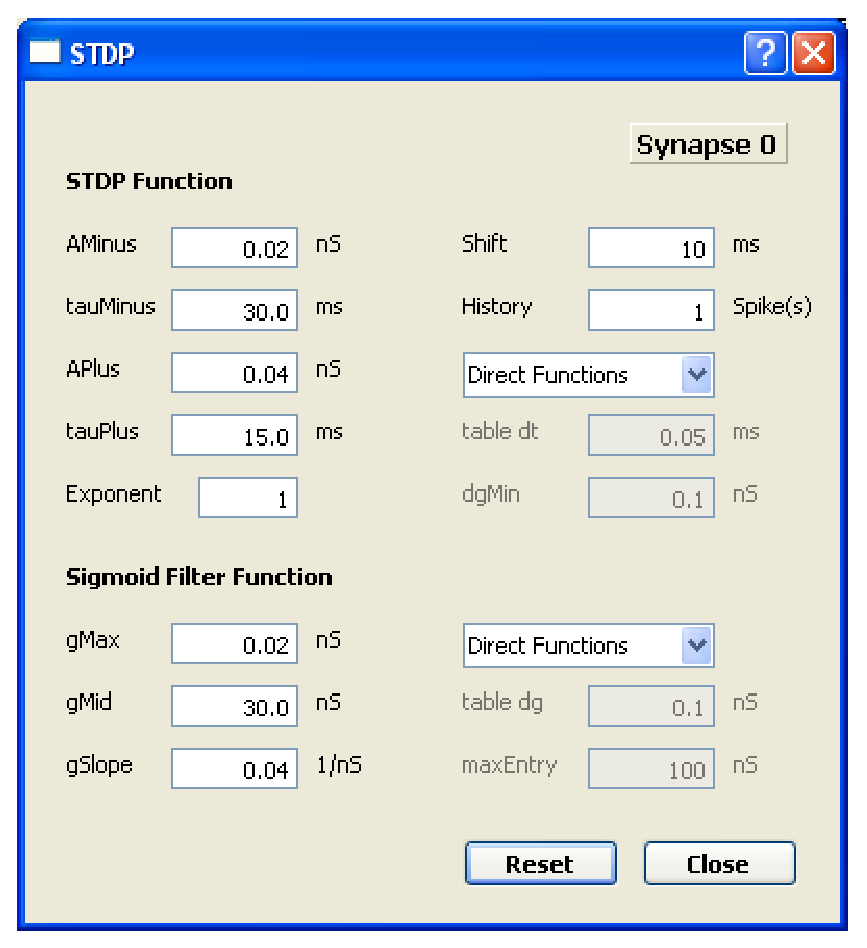
\includegraphics[scale=0.5]{StdpDialog}
}
\hfill
\parbox{0.5\textwidth}{
The control parameters are: \\
``STDP Function''
\begin{myitem}
\item AMinus: The amplitude $A_-$ of the negative (left) part of the STDP curve.
\item tauMinus: The time scale $\tau_-$ (locus of the extremum) of the negative
  (left) part of the STDP curve.
\item APlus: The amplitude $A_+$ of the positive (right) part of the
  STDP curve.
\item tauPlus: The time scale $\tau_+$ (locus of the extremum) of the
  positive (right) part of the STDP curve.
\item Exponent: The exponent $q$ of the polynomial factor in the STDP
  curve. 
\item Shift: The offset $\tau_{\text{Shift}}$ of the STDP curve on the
  $\Delta t$ axis. 
\end{myitem}
}\\
\begin{myitem}
\item History: The number of spikes to be considered in the other
  neuron if a spike occurs in a given neuron. For example, if set to
  $1$ and a spike occurs in the postsynaptic neuron, the change 
  $\Delta g$ will only be calculated and applied for the last spike
  that occurred in the presynaptic neuron. If it was $2$ it would be
  calculated for the last and the next to last spike in the
  presynaptic neuron. Note, history is capped at 20 spikes.
\item The method combo box allows to choose whether the STDP function is
  calculated directly with the appropriate C functions when needed or
  whether it is tabled up front and this lookup-table is being used.
\item table dt: The time step in the lookup table.
\item dgMin: The minimum value for $\Delta g$ that should be in the
  table. This determines how far to the left and right the table
  covers the STDP curve.
\end{myitem}
``Sigmoid Filter Function''
\begin{myitem}
\item gMax: The maximal $g_{\text{Syn}}$ allowed.
\item gMid: The midpoint $g_{\text{Mid}}$ of the filter.
\item gSlope: The ``slope'' parameter $g_{\text{slope}}$ of the sigmoid filter. 
\item The method combo allowing the choice between direct calculation
  or lookup tables for the filter function.
\item table dg: The stepping in terms of $g_{\text{raw}}$ of the
  lookup table.
\item maxEntry: The maximal $g_{\text{raw}}$ entry in the table.
\end{myitem}

\noindent
\emph{Scripting:} Script access to Spike STDP is given through the \texttt{<synapse>.ST} variable.
The following members are available for scripting: \\
\begin{tabular}[b]{|ll|ll|}
	\hline
	{\bf \textless{}synapse\textgreater.ST.\textvisiblespace} & {\bf Value range} 
	& {\bf \textless{}synapse\textgreater.ST.\textvisiblespace} & {\bf Value range} \\
	\hline
	\texttt{AMinus} & double 	& \texttt{Shift} & double \\
	\texttt{tauMinus} & double 	& \texttt{History} & integer [0..20] \\
	\texttt{APlus} & double 	& \texttt{gMax} & double \\
	\texttt{tauPlus} & double & \texttt{gMid} & double \\
	\texttt{Exponent} & integer & \texttt{gSlope} & double \\
	\hline
\end{tabular}\\

Alternatively, if the ``ODE STDP'' option is chosen,
the synaptic strength is governed by a set of differential
equations according to the model of synaptic plasticity in
\cite{Abarbanel2002}. In this case, the maximal synaptic conductance
$g_{\text{Syn}}$ is subject to a differential equation system
\begin{align}
\frac{dP}{dt} = v_{\text{pre}} - \beta_P P \\
\frac{dD}{dt} = v_{\text{post}} - \beta_D D \\
\frac{dg_{\text{raw}}}{dt} = \gamma (P D^\eta - D P^\eta).
\end{align}
The normalized voltages $v_x$ are derived from the measured potentials
$V_x$ through capped linear filters
\begin{align}
v_{\text{pre}} = \left\{ \begin{array}{ll}
0 & V_{\text{pre}} < V_{P,\text{min}} \\
\frac{V_{\text{pre}}-V_{P, \text{min}}}{V_{P, \text{max}}-V_{P,
    \text{min}}} & V_{P, \text{min}}\leq V_{\text{pre}} \leq V_{P,
  \text{max}} \\
1 & V_{P, \text{max}} < V_{\text{pre}} 
\end{array} \right.
\end{align}
and accordingly for $v_{\text{post}}$,
\begin{align}
v_{\text{post}} = \left\{ \begin{array}{ll}
0 & V_{\text{post}} < V_{D,\text{min}} \\
\frac{V_{\text{post}}-V_{D, \text{min}}}{V_{D, \text{max}}-V_{D,
    \text{min}}} & V_{D, \text{min}}\leq V_{\text{post}} \leq V_{D,
  \text{max}} \\
1 & V_{D, \text{max}} < V_{\text{post}} 
\end{array} \right.
\end{align}
\vspace*{0.3cm}

\noindent
\parbox{0.48\textwidth}{
  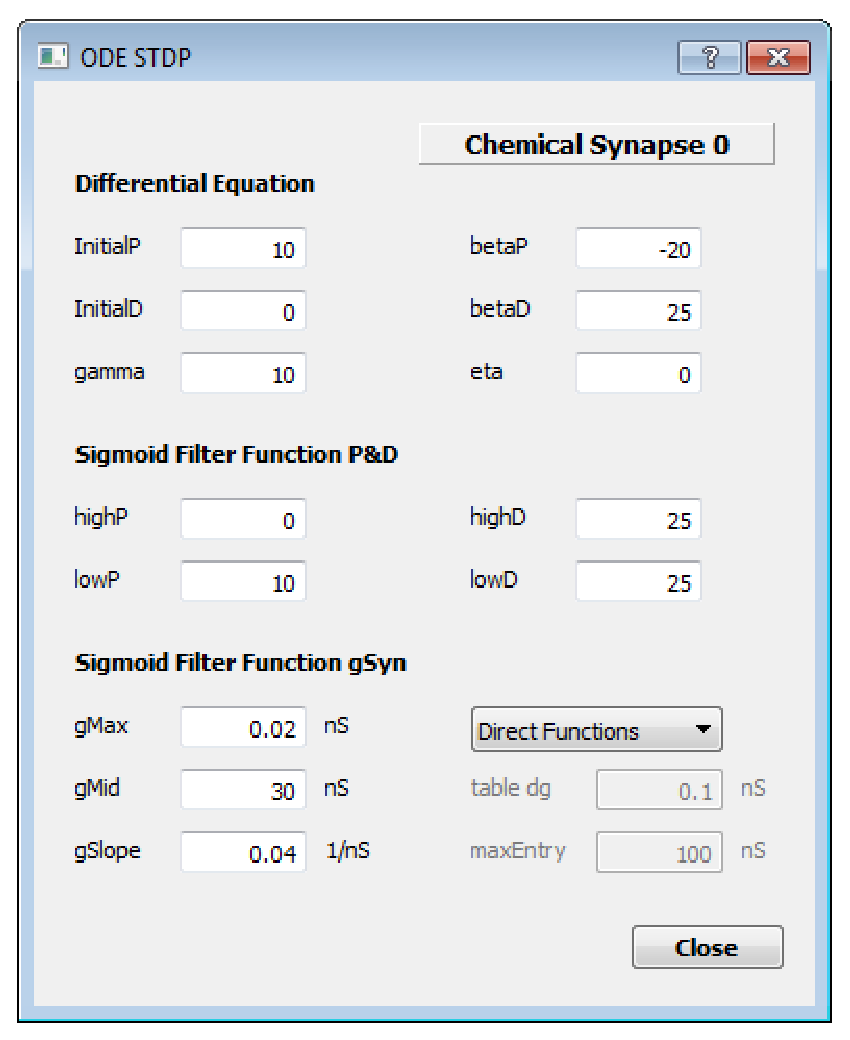
\includegraphics[scale=0.5]{odeStdpDialog} 
}
\hfill
\parbox{0.5\textwidth}{
The control parameters for ODE based STDP are: \\
``Differential Equation''
\begin{myitem}
\item InitialP: Initial value for the ``potentiation variable'' $P$
\item InitialD: Initial value for the ``depression variable'' $D$
\item gamma: Exponent $\gamma$
\item betaP: Rate of decay $\beta_P$ of $P$ in 1/ms= kHz.
\item betaD: Rate of decay $\beta_D$ of $D$ in 1/ms= kHz.
\item eta: Rate of change of $g_{\text{raw}}$ in nS/ms.
\end{myitem}
``Sigmoid Filter Function P \& D''
\begin{myitem}
\item highP: The upper limit $V_{P, \text{max}}$ of the $P$ filter 
\item lowP: The lower limit $V_{P, \text{min}}$ of the $P$ filter 
\item highD: The upper limit $V_{D, \text{max}}$ of the $D$ filter
\item lowD: The lower limit $V_{D, \text{min}}$ of the $D$ filter
\end{myitem}
}\\

``Sigmoid Filter Function gSyn''
\begin{myitem}
\item gMax: The maximal allowed value for $g_{\text{Syn}}$.
\item gMid: The mid point of the sigmoid filter for $g_{\text{Syn}}$
\item gSlope: The ``slope'' parameter of the sigmoid filter function
  for $g_{\text{Syn}}$.
\item The method combo allows to switch between direct evaluation of
  the filter or the use of a lookup table
\item table dg: The step size in the lookup table
\item maxEntry: The maximum of $g_{\text{raw}}$ for which table
  entries are generated.
\end{myitem}  

\noindent
\emph{Scripting:} Script access to ODE STDP is given through the \texttt{<synapse>.ODE} variable.
The following members are available for scripting: \\
\begin{tabular}[b]{|ll|ll|}
	\hline
	{\bf \textless{}synapse\textgreater.ODE.\textvisiblespace} & {\bf Value range} 
	& {\bf \textless{}synapse\textgreater.ODE.\textvisiblespace} & {\bf Value range} \\
	\hline
	\texttt{InitialP} & double 	& \texttt{highP} & double \\
	\texttt{InitialD} & double 	& \texttt{lowP} & integer [0..20] \\
	\texttt{betaP} & double 	& \texttt{highD} & double \\
	\texttt{betaD} & double 	& \texttt{lowD} & double \\
	\texttt{gamma} & double 	& \texttt{gMax} & double \\
	\texttt{eta} & integer 		& \texttt{gMid} & double \\
					 &  		& \texttt{gSlope} & double \\
	\hline
\end{tabular}


\subsection{Ionic Conductances} \label{HHcurrents}

\parbox{\textwidth}{
  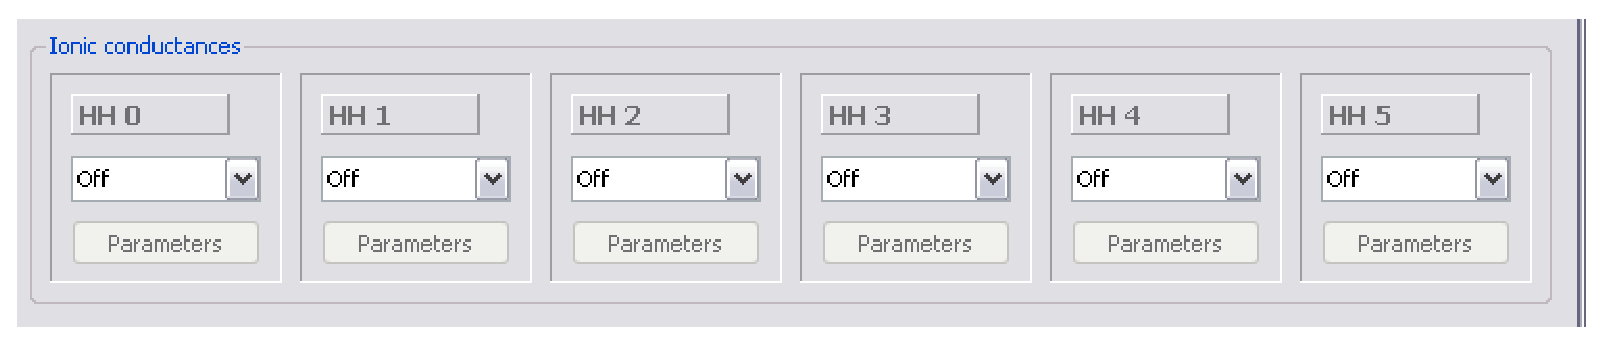
\includegraphics[scale=0.5]{HHBlock}
} \\[0.2cm]

The conductance control block contains an arbitrary number of Hodgkin-Huxley type
conductance configurations.
Conductances are added by selecting the appropriate type in the rightmost box in the
list, labelled ``New...'', and clicking ``Add''. An initially active conductance is
then added to the list, which can be configured by clicking the ``Parameters'' button and
activated or deactivated by checking or unchecking the ``Active'' checkbox. When a conductance is no
longer required, it can be removed by deactivating it and clicking the
``Clear inactive'' button to the right of the list. The ``Reset'' button just below that
resets the entire control block to its last saved state, i.e. the state it was in upon
program start, loading or saving a protocol, or clicking the ``Start'' button.

\subsubsection{m/h/tau Hodgkin-Huxley conductances}

For the ``m/h/tau'' conductance description, the current $I_{HH}$ to be injected
into a cell with membrane potential $V(t)$ is calculated according to
\begin{align}
  I_{HH}(t) = g_{\text{Max}} m(t)^p h(t)^q (V_{\text{rev}}-V(t)),
\end{align}
where $m$ and $h$ are modelled as
\begin{align}
  \tau_m \frac{dm}{dt} &= m_\infty(V)-m , \\
  \tau_h \frac{dh}{dt} &= h_\infty(V)- h, 
\end{align}
with steady state values
\begin{align}
  m_\infty &= \frac{1-C_m}{1+\exp \left(\frac{V - V_m}{s_m}
  \right)}+C_m, \\
  h_\infty &= \frac{1-C_h}{1+\exp \left(\frac{V - V_h}{s_h}
  \right)}+C_h, 
\end{align}
and time scales 
\begin{align}
  \tau_m &= \tau_{0,m} + A_{\tau,m} F_{\tau,m}(V), \\
  \tau_h &= \tau_{0,h} + A_{\tau,h} F_{\tau,h}(V).
\end{align}
The time scale function $F_{\tau,\bullet}$ can be one of the following four choices:
\begin{align}
  \text{``1/(1+exp)''} : F_{\tau,\bullet} &=
    \frac{-1}{1+\exp\left(\frac{V-V_{\tau,\bullet}}{s_{\tau,\bullet}}\right)}, \\
  \text{``tanh\string^2''} : F_{\tau,\bullet} &=
    1 - \tanh^2 \left( \frac{V - V_{\tau,\bullet}}{s_{\tau,\bullet}}\right), \\
  \text{``exp2/(1+exp1)''} : F_{\tau,\bullet} &=
    \exp\left(\frac{V-V_{\tau,\bullet}}{s_{\tau,\bullet}}\right) \bullet_\infty(V), \\
  \text{``Linear''} : F_{\tau,\bullet} &= V.
\end{align}

\noindent
\parbox{0.53\textwidth}{
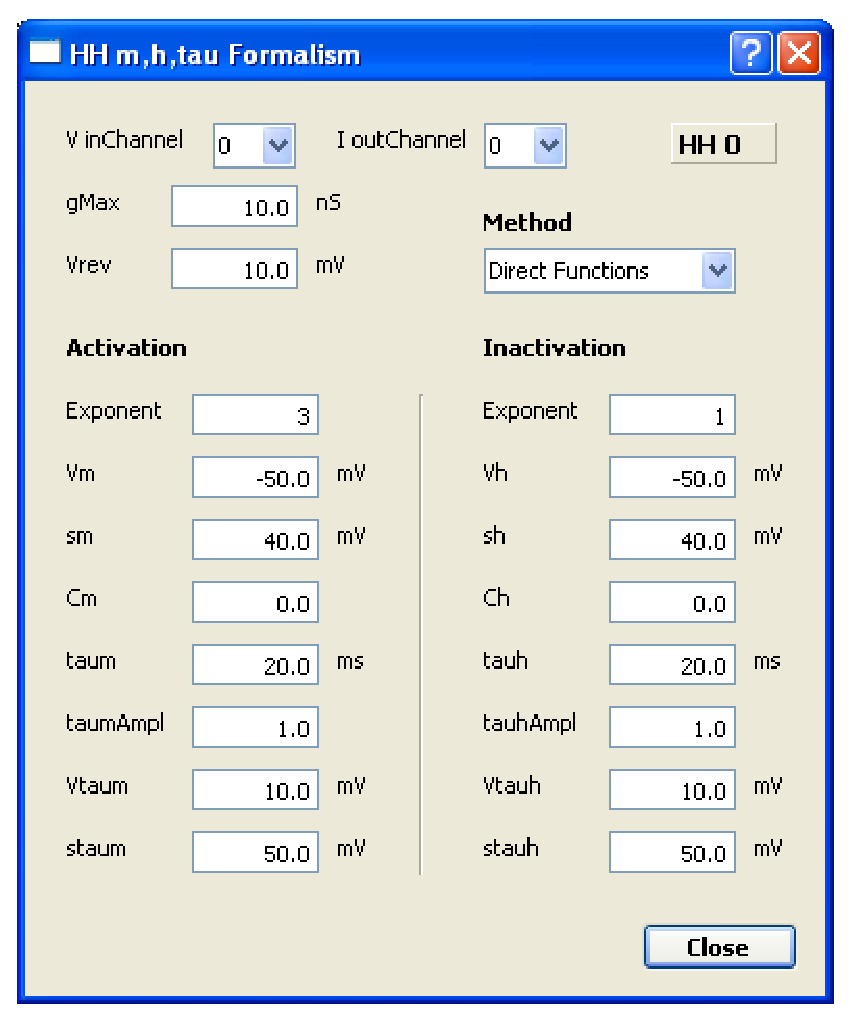
\includegraphics[scale= 0.45]{mhtauDialog}
} 
\hfill
\parbox{0.45\textwidth}{
Control parameters of the ionic conductances in the m/h/tau formalism
are:
\begin{myitem}
\item Channel assignments: Conductances can be assigned to multiple pairs of voltage input (``V in'')
  and current output (``I out'') channels. Each such assignment can be turned on or off individually.
  Assignments to model ``All'' channels are resolved intelligently, such that each active instance of the
  model receives one conductance.
\item gMax: The maximal conductance $g_{\text{Max}}$ of the inserted
  channel
\item Vrev: The reversal potential $V_{\text{rev}}$ of the inserted
  channel
\item Method: The combo box allows to choose between direct evaluation of C
  functions or a pre-calculated lookup table.
\end{myitem}
} \\[0.2cm]

\noindent
``Activation'' and ``Inactivation'' (substituting h for m as appropriate): 
\begin{myitem}
\item Exponent: The exponent $p$ (Activation) or $q$ (Inactivation) in the current equation
\item Vm: The activation potential $V_m$
\item sm: The width $s_m$ of the activation function
\item Cm: The offset parameter $C_m$ for persistent currents
\item taum type: Selects the time scale function $F_{\tau,m}$.
\item taum0: The minimal time scale $\tau_{0,m}$ for $\tau_m$.
\item taumAmpl: The range (Amplitude) $A_{\tau\,m}$ for the time scale $\tau_m$ in ms
 (or, when taum type is ``Linear'', ms/mV).
\item Vtaum: The mid point $V_{\tau,m}$ for the time scale sigmoid function.
\item staum: The ``slope'' parameter $s_{\tau,m}$ for the time scale
sigmoid function  
\end{myitem}

\noindent
\emph{Scripting:} Script access to m/h/tau conductances is given through the \texttt{mhHHp[\#]} variable.
The following members are available for scripting: \\
\begin{tabularx}{\linewidth}{|ll|X|}
	\hline
	{\bf mhHHp[\#].\textvisiblespace} & {\bf Value range} & {\bf Notes} \\
	\hline
	\texttt{active} & 0,1 & Conductances must be initially active. Deactivating a conductance suspends all
	its assignments. \\
	\texttt{assign[\#].active} & 0,1 & Assignments must be initially active. \\
	\texttt{gMax} & double & \\
	\texttt{Vrev} & double & \\
	\texttt{mExpo}, \texttt{hExpo} & integer & Exponent \\
	\texttt{Vm}, \texttt{Vh} & double & \\
	\texttt{sm}, \texttt{sh} & double & \\
	\texttt{Cm}, \texttt{Ch} & double & \\
	\texttt{taumType}, \texttt{tauhType} & 0,1,2,3 & Ordered as above \\
	\texttt{taum}, \texttt{tauh} & double & taum0, tauh0\\
	\texttt{taumAmpl}, \texttt{tauhAmpl} & double & Units: For linear tau type, the value is
	interpreted as s/mV, otherwise as s.\\
	\texttt{Vtaum}, \texttt{Vtauh} & double & \\
	\texttt{staum}, \texttt{stauh} & double & \\
	\hline
\end{tabularx}

\subsubsection{Alpha-Beta Hodgkin-Huxley conductances}

\noindent
Alternatively, the ionic conductances can be described in a
$\alpha$/$\beta$ formalism, where
\begin{align}
I_{\text{HH}}= g_{\text{Max}} m^p h^q (V_{\text{rev}}-V) \\
\frac{dm}{dt}= \alpha_m (1-m) - \beta_m m \\
\alpha_m= k_{\alpha,m} F_{\alpha,m}\left(\frac{V-V_{\alpha,m}}{s_{\alpha,m}}
\right) \\
\beta_m= k_{\beta,m} F_{\beta,m}\left(\frac{V-V_{\beta,m}}{s_{\beta,m}}
\right) \\
\frac{dh}{dt}= \alpha_h (1 - h) - \beta_h h \\
\alpha_h= k_{\alpha,h} F_{\alpha,h}\left(\frac{V-V_{\alpha,h}}{s_{\alpha,h}}
\right) \\
\beta_h= k_{\beta,h} F_{\beta,h}\left(\frac{V-V_{\beta,h}}{s_{\beta,h}}
\right).
\end{align}
The ``activation'' and ``inactivation'' functions $F_{\bullet , \bullet}$ can
be chosen from three options,
\begin{align}
\text{``k*V/(exp(V)-1)''} : F_{\bullet , \bullet}(x) &= \frac{x}{\exp(x)-1} \\
\text{``k*exp(V)''} : F_{\bullet , \bullet}(x) &= \exp(x) \\
\text{``k*1/(1+exp(V))''} : F_{\bullet , \bullet}(x) &= \frac{1}{1+\exp(x)}.
\end{align}
Note that this formalism allows you to implement, for example, the classic
neuron model by Traub and Miles \cite{Traub1991}. \\

\noindent
\parbox{0.54\textwidth}{
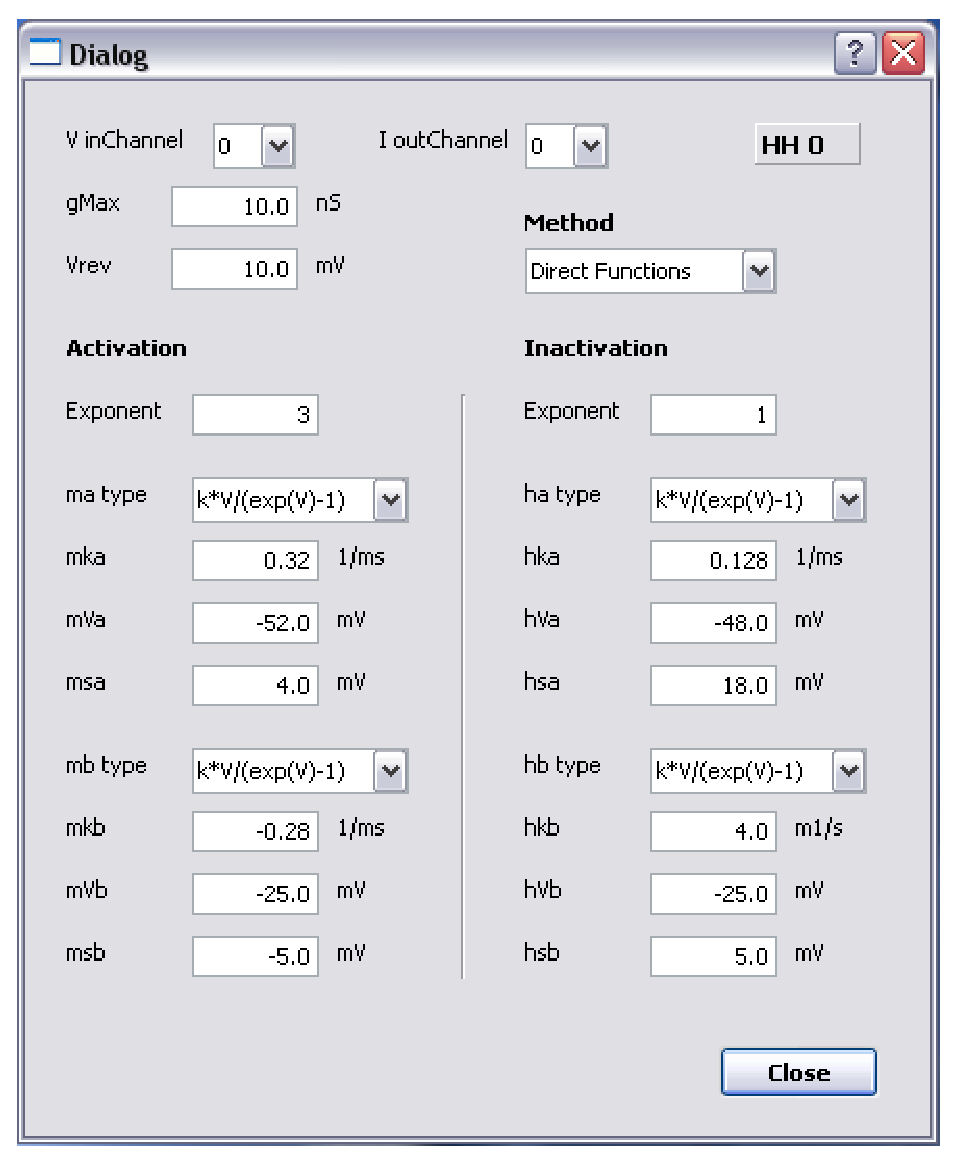
\includegraphics[scale= 0.45]{alphaBetaDialog}
}
\hfill
\parbox{0.45\textwidth}{
The control parameters are
\begin{myitem}
\item Channel assignments, gMax, Vrev, Method as above;
\end{myitem}
``Activation'' and ``Inactivation'' (substituting h for m as appropriate):
\begin{myitem}
	\item Exponent: The exponent $p$ (Activation) or $q$ (Inactivation) in the current equation
	\item ma type: The choice of the functional form for $F_{\alpha,m}$.
	\item mka: Rate parameter $k_{\alpha,m}$ for the rise of $m$
	\item mVa: The midpoint $V_{\alpha,m}$ for the sigmoid function
	for $\alpha_m$ 
	\item msa: The ``slope'' parameter $s_{\alpha,m}$ for the sigmoid function
	for $\alpha_m$
	\item mb type: The choice of the functional form for $F_{\beta,m}$.
	\item mkb: Rate parameter $k_{\beta,m}$ for the decay of $m$
\end{myitem}
} 
\begin{myitem}
	\addtocounter{enumi}{7}
	\item mVb: The midpoint $V_{\beta,m}$ for the sigmoid function
	for $\beta_m$ 
	\item msb: The ``slope'' parameter $s_{\beta,m}$ for the sigmoid function
	for $\beta_m$
\end{myitem}

\noindent
\emph{Scripting:} Script access to alpha-beta conductances is given through the \texttt{abHHp[\#]} variable.
The following members are available for scripting: \\
\begin{tabularx}{\linewidth}{|ll|X|}
	\hline
	{\bf abHHp[\#].\textvisiblespace} & {\bf Value range} & {\bf Notes} \\
	\hline
	\texttt{active} & 0,1 & Conductances must be initially active. Deactivating a conductance suspends all
	its assignments. \\
	\texttt{assign[\#].active} & 0,1 & Assignments must be initially active. \\
	\texttt{gMax} & double & \\
	\texttt{Vrev} & double & \\
	\texttt{mExpo}, \texttt{hExpo} & integer & Exponent \\
	\texttt{maFunc}, \texttt{mbFunc}, \texttt{haFunc}, \texttt{hbFunc} & 0,1,2 & Activation/inactivation 
	functions, ordered as above. \\
	\texttt{mka}, \texttt{mkb}, \texttt{hka}, \texttt{hkb} & double & \\
	\texttt{mVa}, \texttt{mVb}, \texttt{hVa}, \texttt{hVb} & double & \\
	\texttt{msa}, \texttt{msb}, \texttt{hsa}, \texttt{hsb} & double & \\
	\hline
\end{tabularx}


\subsection{Tools}

\noindent
\parbox{\textwidth}{
	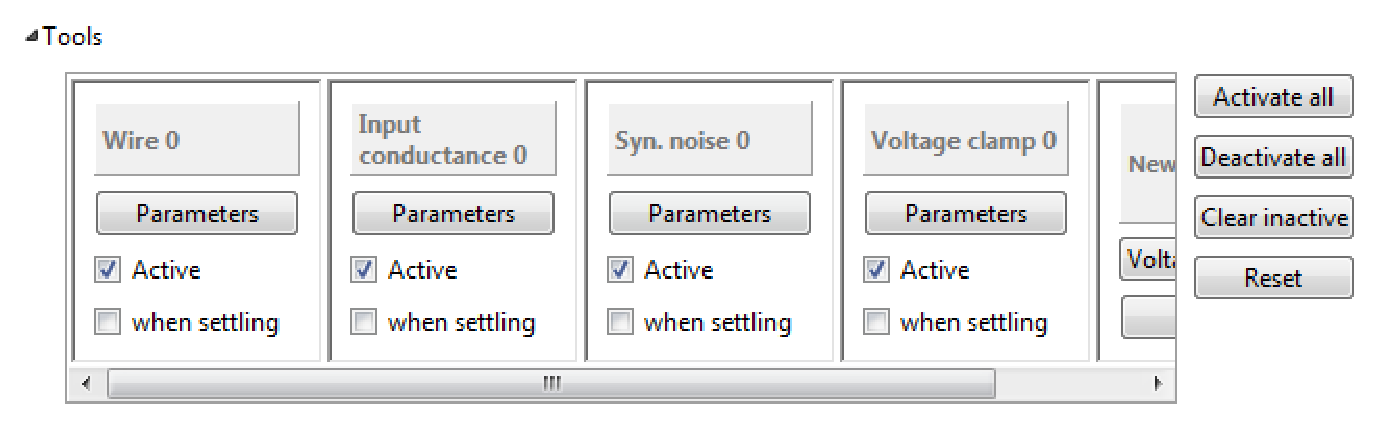
\includegraphics[scale=0.6]{tools}
} \\[0.2cm]

\subsubsection{Wire}
The wire tool is a very simple module that writes data from an input channel (e.g. from an acquisition
device, from the spike generator, or similar) to an existing output channel. This circumvents StdpC's
separation of input and output channels and may be useful in various non-standard use cases.
Other than channel assignments, this module has only one functional parameter, namely a conversion factor.

\noindent
\emph{Scripting:} Script access to the Wire module is given through the \texttt{Wire[\#]} variable.
The following members are available for scripting: \\
\begin{tabularx}{\linewidth}{|ll|X|}
	\hline
	{\bf Wire[\#].\textvisiblespace} & {\bf Value range} & {\bf Notes} \\
	\hline
	\texttt{active} & 0,1 & Modules must be initially active. Deactivating a module suspends all
	its assignments. \\
	\texttt{assign[\#].active} & 0,1 & Assignments must be initially active. \\
	\texttt{factor} & double & The factor k used to calculate the output as $I=kV$.\\
	\hline
\end{tabularx}

\subsubsection{Input conductance}
\noindent
\parbox{\textwidth}{
	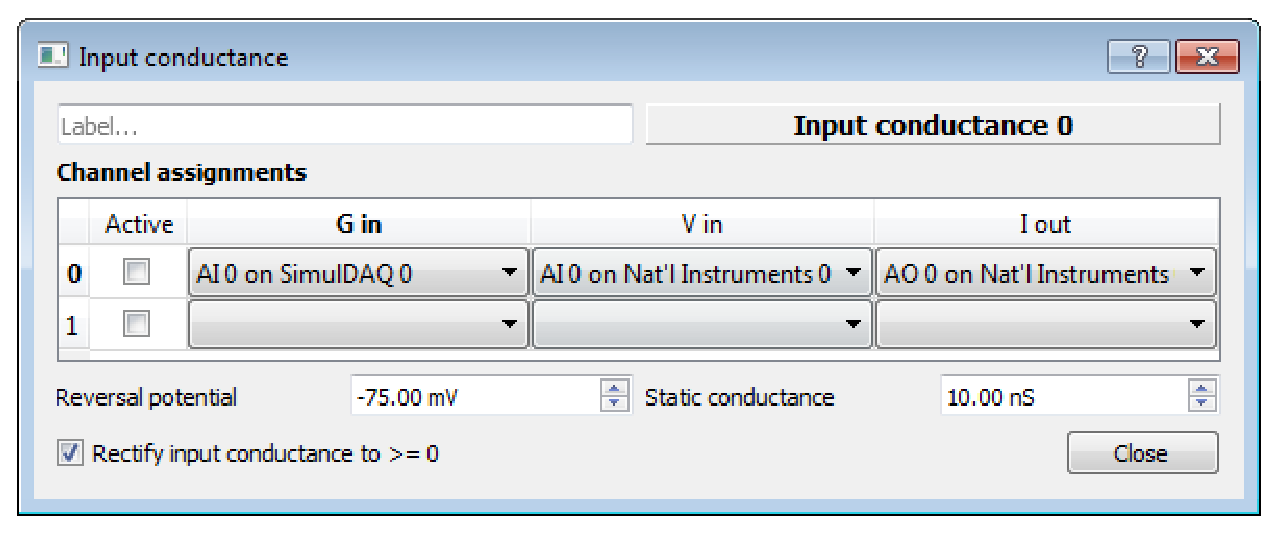
\includegraphics[scale=0.5]{inputConductance}
} \\[0.2cm]
The \emph{Input conductance} tool can be used to inject an externally defined conductance waveform
into a membrane. That is, rather than calculating the conductance according to a model, as the synapse
and ionic conductance modules do, the conductance value is taken from an input channel,
labelled ``G in'' in the channel assignments. For example, one might use a SimulDAQ input file to
describe a conductance time series. The following controls are available:
\begin{myitem}
	\item Reversal potential: The reversal potential of the conductance.
	\item Static conductance: Conversion factor k applied to the samples read from ``G in''. That is,
	the resulting current is defined as $I(t) = k G(t) (V_{\text{rev}} - V_{\text{in}}(t))$.
	\item Rectify input conductance to $\geq 0$: If checked, any negative \emph{conductance} values read
	from the ``G in'' channel are interpreted as zero. Note, this is not rectification of the current,
	only of the conductance.
\end{myitem}

\noindent
\emph{Scripting:} Script access to input conductances is given through the \texttt{InputCond[\#]} variable.
The following members are available for scripting: \\
\begin{tabularx}{\linewidth}{|ll|X|}
\hline
{\bf InputCond[\#].\textvisiblespace} & {\bf Value range} & {\bf Notes} \\
\hline
\texttt{active} & 0,1 & Modules must be initially active. Deactivating a module suspends all
its assignments. \\
\texttt{assign[\#].active} & 0,1 & Assignments must be initially active. \\
\texttt{Vrev} & double &\\
\texttt{gStatic} & double &\\
\texttt{rectify} & 0,1 &\\
\hline
\end{tabularx}

\subsubsection{Synaptic noise}
The synaptic noise module injects a pseudo-random conductance designed to mimic synaptic background noise,
following the model proposed by \cite{destexhe2001fluctuating}. A single (inhibitory or excitatory)
synaptic background noise current with a reversal potential $V_{\text{rev}}$ is calculated as follows:
\begin{align}
I(t) &= g(t) (V_{\text{rev}} - V_{\text{in}}(t)) \\
g(0) &= \bar{g} \\
g(t + \Delta t) &= \bar{g} + (g(t) - \bar{g}) e^{-\Delta t/\tau}
 + R \sqrt{\frac{D\tau}{2}(1 - e^{-2\Delta t/\tau})} \\
R &\sim N(0,1) \\
D &= \frac{2\sigma^2}{\tau}
\end{align}

\noindent
\parbox{0.59\textwidth}{
	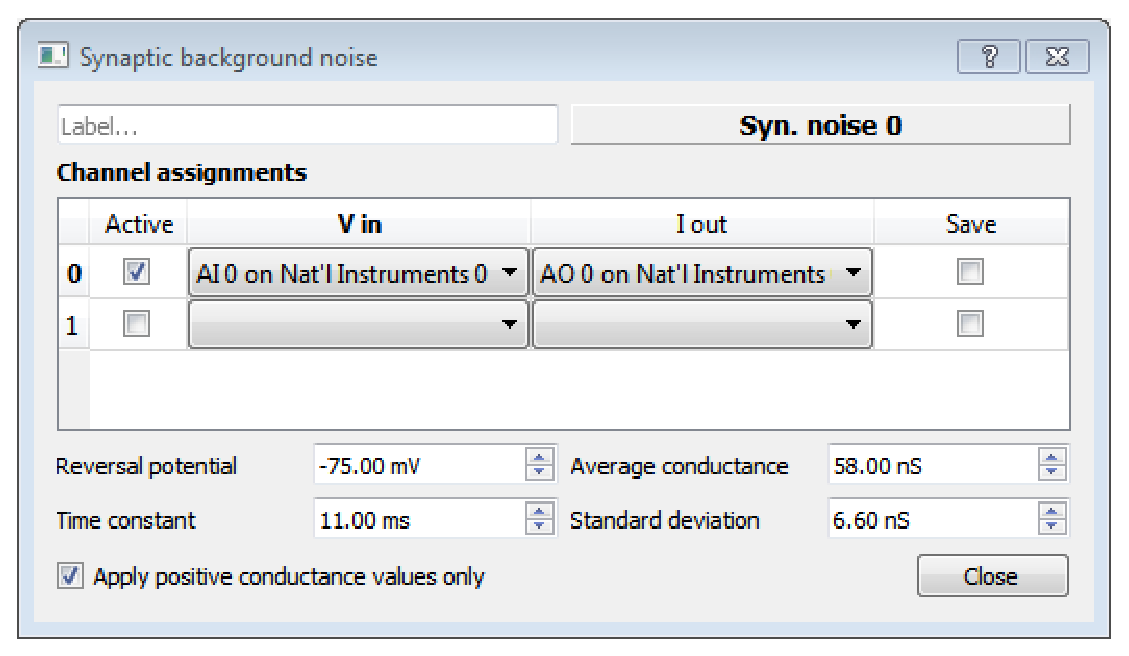
\includegraphics[scale=0.45]{SynapticNoise}
}
\hfill
\parbox{0.4\textwidth}{
The following parameters are available:
\begin{myitem}
	\item Reversal potential: $V_{\text{rev}}$ in the above equations.
	\item Time constant: $\tau$ in the above equations. The time constant determines the noise quality,
	ranging from purely white noise ($\tau = 0$) to coloured noise that looks more like Brownian motion
	($\tau > 0$).
\end{myitem}
}
\begin{myitem}
	\item Average conductance: $\bar{g}$ in the above equations. The actual conductance will fluctuate
	around this value.
	\item Standard deviation: $\sigma$ in the above equations. This determines how widely the conductance
	fluctuates.
	\item Apply positive conductance values only: Check to rectify the applied conductance and avoid
	physically impossible negative conductances. Note that $g(t)$ may fluctuate into negative values
	regardless, but with this setting turned on, $g(t) < 0$ implies $I(t) = 0$.
\end{myitem}

\noindent
\emph{Scripting:} Script access to synaptic noise conductances is given through the
 \texttt{SynapticNoisep[\#]} variable. The following members are available for scripting: \\
\begin{tabularx}{\linewidth}{|ll|X|}
\hline
{\bf SynapticNoisep[\#].\textvisiblespace} & {\bf Value range} & {\bf Notes} \\
\hline
\texttt{active} & 0,1 & Modules must be initially active. Deactivating a module suspends all
its assignments. \\
\texttt{assign[\#].active} & 0,1 & Assignments must be initially active. \\
\texttt{Vrev} & double &\\
\texttt{tau} & double &\\
\texttt{g0} & double & The average conductance $\bar{g}$.\\
\texttt{std} & double & The standard deviation $\sigma$.\\
\hline
\end{tabularx}

\subsubsection{Voltage clamp}
This is an experimental software-defined voltage clamp implementation, using PID control to achieve
voltage clamp e.g. in absence of a suitable amplifier, or -- depending on the system used
-- possibly with better control characteristics. The module takes a command voltage input (``Command V'')
and calculates a control current (``Clamp I'') based on the measured membrane potential (``Cell V'').
Control current is the sum of proportional, integral and differential components $I_p$, $I_i$ and $I_d$,
defined as follows:
\begin{align}
I_p &= g_p(V_\text{cmd} - V_m)\\
I_i &= g_i(\bar{V}_\text{cmd} - \bar{V}_m)\\
I_d &= g_d(\frac{dV_\text{cmd}}{dt} - \frac{dV_m}{dt})
\end{align}
The running averages $\bar{V}_\text{cmd}$ and $\bar{V}_m$ are calculated using a decay factor $k$, such
that $\bar{V}(t + \Delta t) = k\bar{V}(t) + V(t)$. The differential voltages $dV/dt$ are approximated at
each time step using the difference between $V(t)$ and the voltage \emph{tD} steps previous.

Besides these parameters, the module supports an ease-in period during which the total current output is
multiplied with a linearly increasing factor, starting from 0 at the start of clamping to 1 at the end
of ease-in. During this period, if the total current amplitude exceeds the given limit, the voltage clamp
module is deactivated to protect the cell against damage from ringing. \\[0.2cm]

\noindent
\parbox{\textwidth}{
	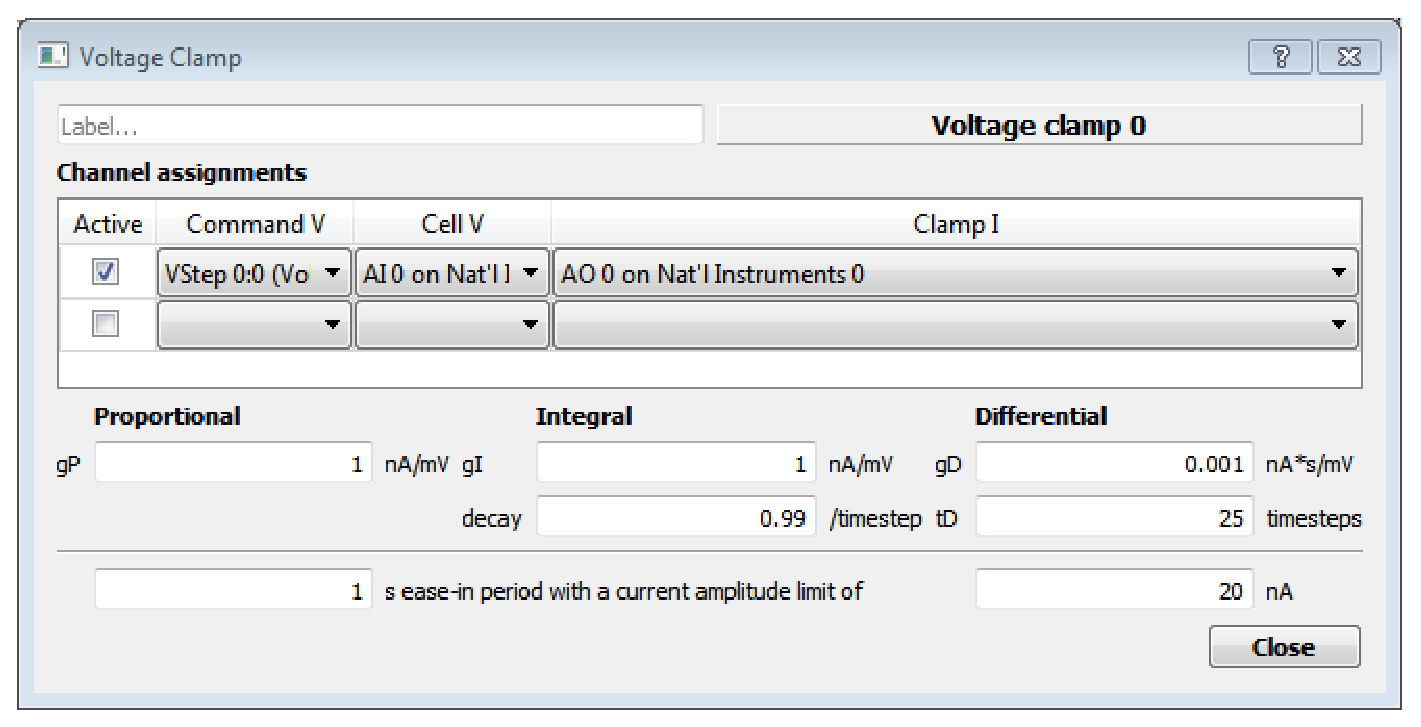
\includegraphics[scale=0.5]{VClamp}
} \\[0.2cm]

\noindent
\emph{Scripting:} Script access to the voltage clamp module is given through the
\texttt{VoltageClamp[\#]} variable. The following members are available for scripting: \\
\begin{tabularx}{\linewidth}{|ll|X|}
\hline
{\bf VoltageClamp[\#].\textvisiblespace} & {\bf Value range} & {\bf Notes} \\
\hline
\texttt{active} & 0,1 & Modules must be initially active. Deactivating a module suspends all
its assignments. \\
\texttt{assign[\#].active} & 0,1 & Assignments must be initially active. \\
\texttt{gP}, \texttt{gI}, \texttt{gD} & double &\\
\texttt{decayI} & double & Decay factor per time step.\\
\texttt{easeIn} & double & Ease-in time; note that linear interpolation always starts from t=0.\\
\texttt{easeInAmpLimit} & double &\\
\hline
\end{tabularx}

\subsection{Data display}
The data display in StdpC is very useful to check the parameter
settings chosen. Typical errors in dynamic clamp setups are wrong
conversion factors on input and output channels. By displaying the
data acquired on input channels in the graph displays, some of these
errors can easily be detected and corrected. On reasonably modern
hardware (i.e., any computer with multiple processor cores), graphing
should have very little impact on clamp cycle performance. \\[0.2cm]
\parbox{\textwidth}{
  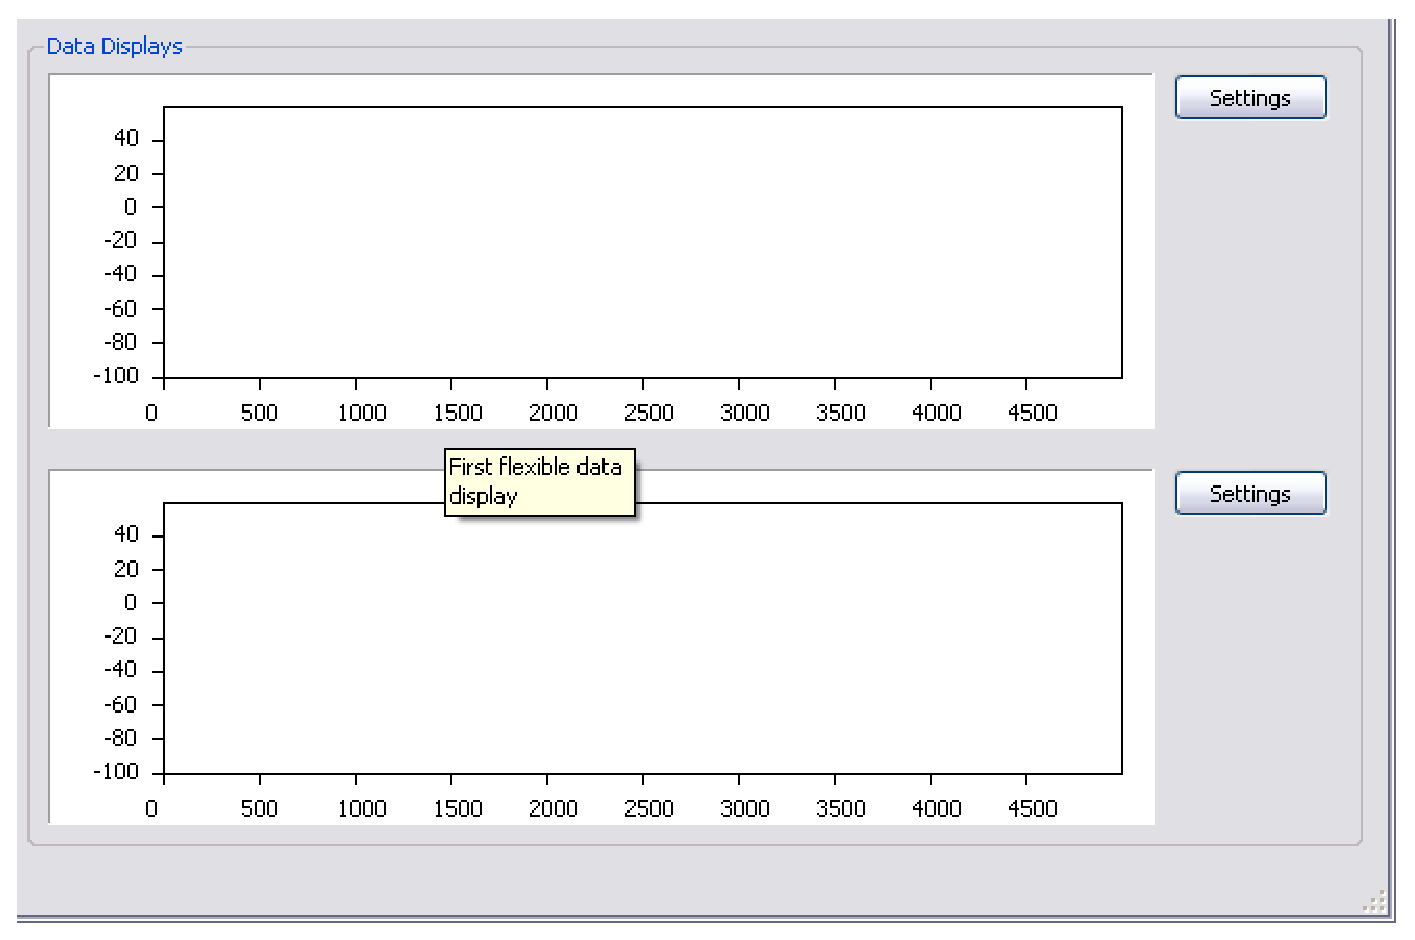
\includegraphics[scale=0.6]{graphBlock}
} \\[0.2cm]

The graph panel control elements are:
\begin{myitem}
\item Sampling interval: Sets the graph sampling frequency that StdpC aims for.
The achieved sampling frequency is displayed to the right and is usually a little
smaller than the desired rate.
\item Buffer size: Sets the number of samples that can be held in each trace's buffer.
It may be necessary to increase this for high sampling rates. Tell-tale signs of a
buffer overflow are gaps in the data, which appear as straight line segments,
interspersed with smooth curve sections.
\end{myitem}

To select channels for plotting, click ``New plot'' or double-click an existing plot to bring up
the plot configuration dialog. All input and output channels as well as raw conductance values are
available for plotting. All graphs are plotted on the same axis, but can be scaled by selecting an
appropriate unit modifier.

The data display is controlled with the mouse. To zoom in or out, use the scroll
wheel while mousing over the display. To move the plot, click and drag it. You can also select
each of the axes by clicking them (the axis will turn blue) in order to zoom/drag along
this axis only. Individual traces can be hidden by clicking their legend entry. The height of a plot
can be adjusted along the left edge.
These data display adjustments can be made at any time and do not interfere with the data displayed.

\subsection{Performance monitor}

The performance monitor is a valuable diagnostic tool which displays the
average clamp cycle duration, as well as best and worst case markers. The performance
monitor has two control elements; a checkbox to enable the monitor, and an input to
set the sampling interval. Worst case, best case and mean cycle duration are all
computed with regards to the sampling interval. \\[0.2cm]
\parbox{\textwidth}{
	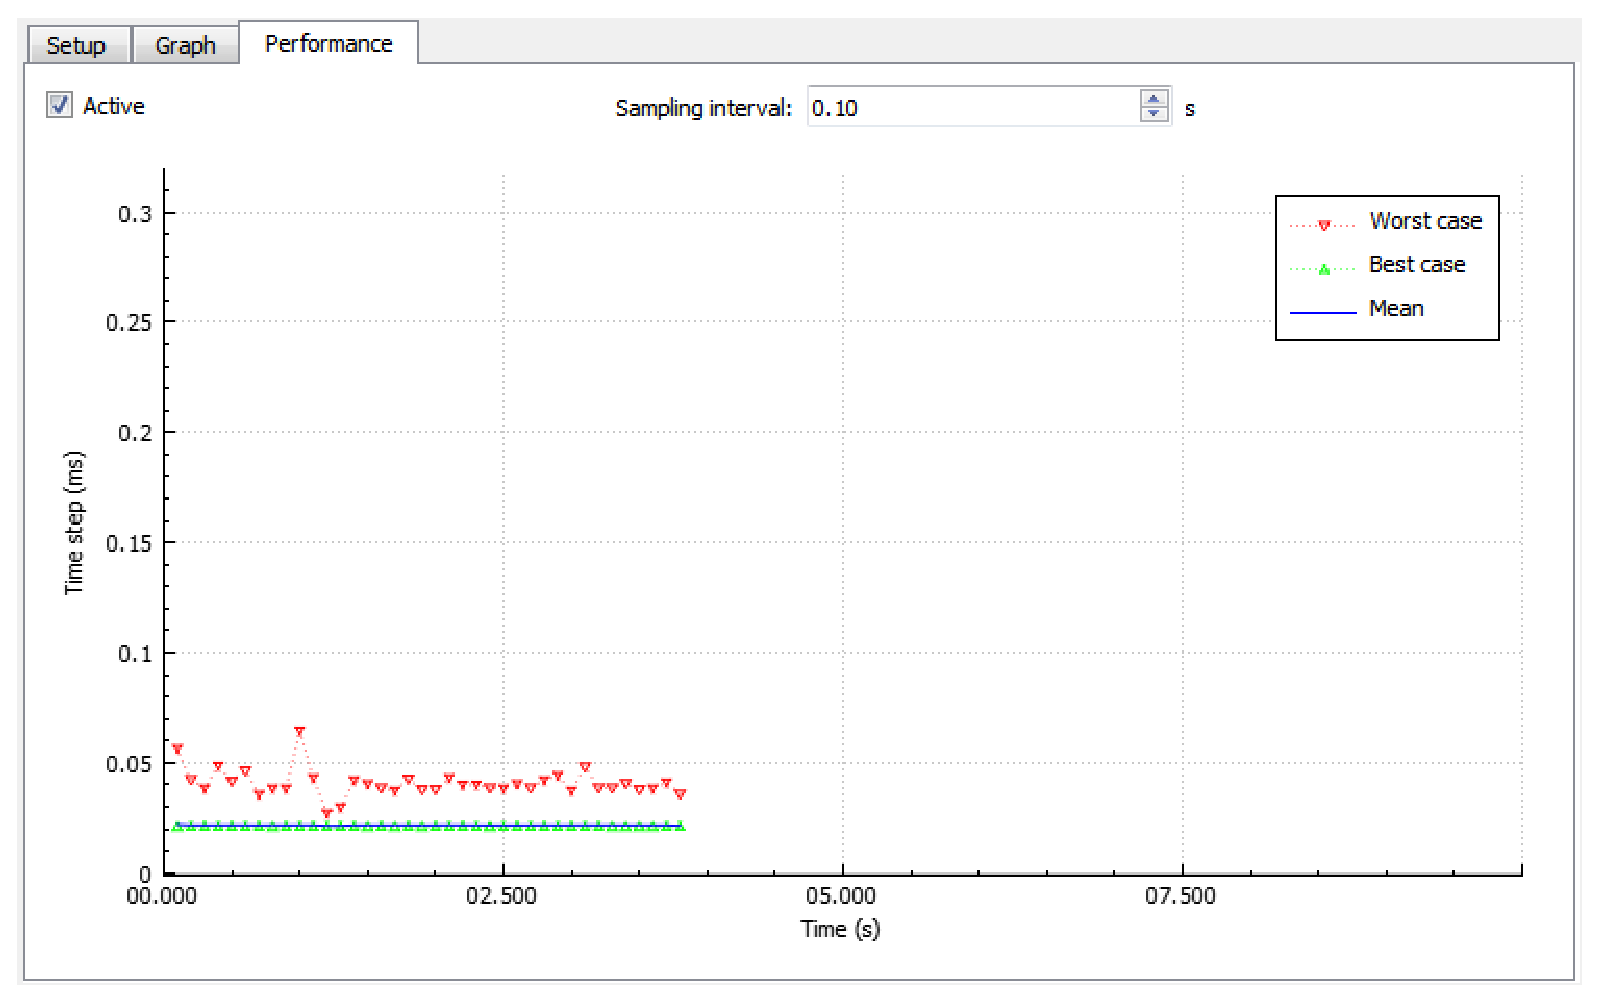
\includegraphics[scale=0.6]{performanceMonitor}
} \\[0.2cm]


\section{Experiment automation} \label{scriptsect}

So far we have described how to control StdpC using the graphical
user interface. Instead, or in addition, most parameters can be
controlled through a scripting mechanism. Through the
File $\rightarrow$ Load Script one can specify a script file. The script
file should contain three columns:
\begin{myenum}
\item A time in seconds when a certain event shall occur
\item A parameter name in clear text which shall be changed
\item A new value for the parameter in question
\end{myenum}
The value column can contain double precision numbers or integers
depending on the parameter being changed.

The script file will be read into a list of events in memory such that
changes to the file have no effect after the script was loaded.

The parameter names are the same as used when the state of the GUI is
saved (``save protocol''), and are listed in the relevant sections above.
Note that protocols contain further parameters that cannot be changed
while the clamp is running, and which are therefore not listed above.
Their inclusion in a script file is discouraged and may lead
to unexpected behaviour.

Please note that in script and protocol files, all parameters and variables are in SI
units V, A, s, S, etc. unless noted otherwise.


\section{Electrode compensation} \label{eleccomp}

For the compensation of electrode artifacts, StdpC uses the so-called Active
Electrode Compensation (AEC) algorithm, developed by Romain Brette and his 
colleagues. Here we only discuss those parts of this cutting-edge
compensation technique, that are necessary for the StdpC end-user to be aware of,
however we also encourage the user to consult \cite{Brette2008} 
and its supplementary material for the full description of the algorithm.

The AEC method consist of two parts: an initial calibration phase and the
subsequent compensation phase happening during the actual experiment. The
first part is the calibration phase, during which StdpC first
injects a probing current into the cell (which is an uncorrelated white noise
signal), and records the voltage response of the system (comprising of
the cell and the electrode) to that current. Based on the
acquired signal-response relationship, the software then calculates the actual parameter
values of the used electrode for the general AEC model. Having had the
electrode calibrated, in the second phase, StdpC automatically uses
this digital model of the electrode on the corresponding input channel, and
calculates the artefactual voltage drop across the electrode occurring on
the recording of that channel due to current injection through the electrode.

\subsection{Basic considerations and troubleshooting for electrode compensation}

High fidelity artifact compensation requires well-calibrated
electrodes, thus the calibration phase is a crucial part of the electrode
compensation process. Even though it is implemented in the most automated
way possible, there are several points the user must make sure before
calibration and take care after calibration (just like in the case of any other
calibration technique). Briefly these are the
following (see \cite{Brette2008} Supp. Mat. for details): 
\begin{myitem}
\item \emph{Do the calibration only when the electrode is already in the
  cell.} Electrode properties change after cell membrane impalement, and
  the electrode has to be calibrated in its stable state.
\item \emph{Make sure that the electrode is (sufficiently) linear in terms
  of its steady state resistance.} One of 
  the basic assumptions of AEC is that the steady state electrode voltage
  response changes linear with the amplitude of the current level injected
  into it. The Electrode Compensation dialog has a built-in feature to
  assess the linearity of the electrode (see below). If you experience too
  high deviation in the steady-state voltage levels in response to
  different voltage levels (e.g. above 10\% of the electrode resistance),
  we recommend to change the electrode, and rerun the linearity test for
  the new one.
\item \emph{Make sure that the electrode has reached an equilibrium state
  in terms of its steady state resistance before calibration.} During
  experiment, any change in the electrode properties after calibration
  would result in an error in the artifact compensation. The most varying
  property is the resistance of the electrode, which can change remarkably
  especially in the first few minutes after cell
  impalement. Thus one must always make sure that the steady-state
  electrode resistance is not changing any more before calibration. The
  electrode measurement feature on the Electrode Compensation dialog
  provides a convenient way for this assessment (see below).  
\item \emph{Make sure that the electrode is at least ten times faster than
  the cell membrane.} Another basic assumption of the AEC calibration phase
  is that the electrode and the passive cell membrane (ie. not spiking, but
  subthreshold) responses are separable in the time domain. This usually satisfied in general
  electrode/cell configurations, but does not stand in case of a very slow
  electrode and a very fast cell membrane. The Electrode Calibration dialog
  provides means for the measurement of both electrode and cell membrane
  response properties (resistance levels, time constants and their standard
  deviations, see below). As in the case of large cells it can
  be difficult to effectively drive and measure the cell's subthreshold properties,
  generally one can satisfy this criterion by making sure that the electrode
  time constant (which can be measure more reliably) is around half
  millisecond or less. If the electrode has been found too
  slow, one can use a certain level of capacitance neutralization (CN)
  during the calibration and the compensation. This CN level must be set before
  calibration, and left unchanged during the usage of the same calibrated
  model of the electrode. See also next point for applying CN.
\item \emph{Turn other compensation techniques off before calibration and
  during compensation as well.} AEC is a complete
  electrode compensation method. The simultaneous operation of any
  other active electrode compensation technique, like bridge balancing or
  discontinuous injection/recoding, would lead to disastrous compensation
  results. The only exception from this rule is the capacitance neutralization
  feature of many microelectrode amplifier, which is able to increase the artifact
  compensation fidelity of AEC, if it is carefully set to the maximum
  possible level before calibration and left unchanged during the
  experiment (see previous point).
\item \emph{Assess actual data acquisition frequency after calibration.}
  Right after calibration the user should make sure that StdpC had been
  able to run the data acquisition part of the compensation in a relatively
  constant frequency by observing the \emph{Std in sampling rate} text
  field in the \emph{Data acquisition results} subpanel (in the bottom
  right corner). The software automatically warns the user if this
  deviation is higher than 0.01, what results in a degradation in the
  quality of the electrode calibration and thus in the subsequent artifact
  compensation as well. Most of the time the popping up of this warning
  means that a significant operation system interruption has occurred
  during calibration (it is also possible that the hardware (PC and/or DAQ)
  is not able to reach the required sampling rate set in the top right
  corner, in which case lowering the rate should solve the issue). To avoid
  the operation system interruption problem, and also to reach the best
  clamping quality, we strongly recommend to stop
  all computational intensive processes the computer might run in the
  background during calibration and dynamic clamping.
\item \emph{Recalibrate if electrode properties has changed over time.} As
  for all electrode artifact compensation technique, the compensation quality
  degrades if changes in the electrode properties (mostly in the
  resistance) have occured as a long experiment goes on. To rule out this
  possibility, we recommend the check of the electrode resistance or even
  the recalibration of the electrode from time to time during the
  experiment, and also the assessment of the electrode after the
  experiment has finished to validate the quality of the compensation. 
\end{myitem}

\subsection{Supported features and the dialog panel}

Along with the electrode calibration, the Electrode Compensation dialog has
two auxiliary features to facilitate calibration and subsequent
artifact compensation at high quality. 

The \emph{electrode measurement} feature acquires the electrode resistance
and time constants according to a simple parallel RC circuit model by
injecting different constant current levels into the electrode and
simultaneously recording the onset-dynamic and equilibrium level of the
voltage response. There are three important things to assess here: (1) the
electrode is fast enough (ie. that its average time constant is less then
about 1 ms), (2) the electrode is linear enough (ie. that the standard
deviation in its resistance levels at different current levels is below
10\% of its absolute average resistance), and (3) the electrode has reached
an equilibrium level in its resistance (ie. the average electrode
resistance does not change remarkably in between subsequent
measurements). Also see the troubleshooting subsection above for a more
detailed discussion of these issues. It is crucial to find a long enough,
but not too long injection length while the electrode is in the cell, in
order to let the electrode reach its steady state voltage response, but in
the same also time prevent the cell membrane to markedly influence the
measurement of the electrode characteristics. A rule of thumb is to set the
injection length between 3 and 5 times of the expected electrode time
constant, what usually leads to injection lengths around 1 and 2 ms. An
incidental spike of the cell simultaneously with the electrode measurement
always result in incorrectly measured properties, this case the one should
remeasure the electrode. 

The \emph{cell membrane measurement} feature allows for the measure of the
same (passive) properties of the cell membrane, based on the same parallel
RC model of the membrane and the already acquired electrode
characteristics. This measurement is done by injecting a particular current step
into the cell, holding it for a certain duration, then stepping back to
zero current level, waiting for the same amount of time to allow the membrane
potential to recover, and then doing the same injection/waiting cycle for a
user-settable number of times. This feature is included to allow the user
to get a rough idea about the time constant of the cell membrane and this
way the appropriateness of the electrode for AEC (the electrode must be at
least 10 times faster than the passive cell membrane for good quality
artifact compensation) Also see the troubleshooting subsection above for a
more detailed discussion of this issues. Please be aware, that because of
the nature of measurement protocol, it is likely to provide good cell properties,
only if (1) the electrode has been measured previously and its resistance
has not changed significantly meanwhile, (2) the passive membrane response
is at least one order of 
magnitude slower than the electrode (only required for precise membrane time
constant calculation), and most importantly (3) the injected current is
able to effectively drive the membrane potential of the cell, that is,
no indenpendent activity of the cell (let it be sub- or suprathreshold)
intervene and contaminate the measurement remarkably. This last point
implies that successful membrane property measurement of large cells
probably requires high amplitude currents, if it is possible at all with
this technique. As large cells usually have slower membrane, in these cases
the user can satify the ``time-separability'' criterion (see
Troubleshooting section) by making sure that they do not use a very slow
electrode (ie. time constant is lower than 1ms).  



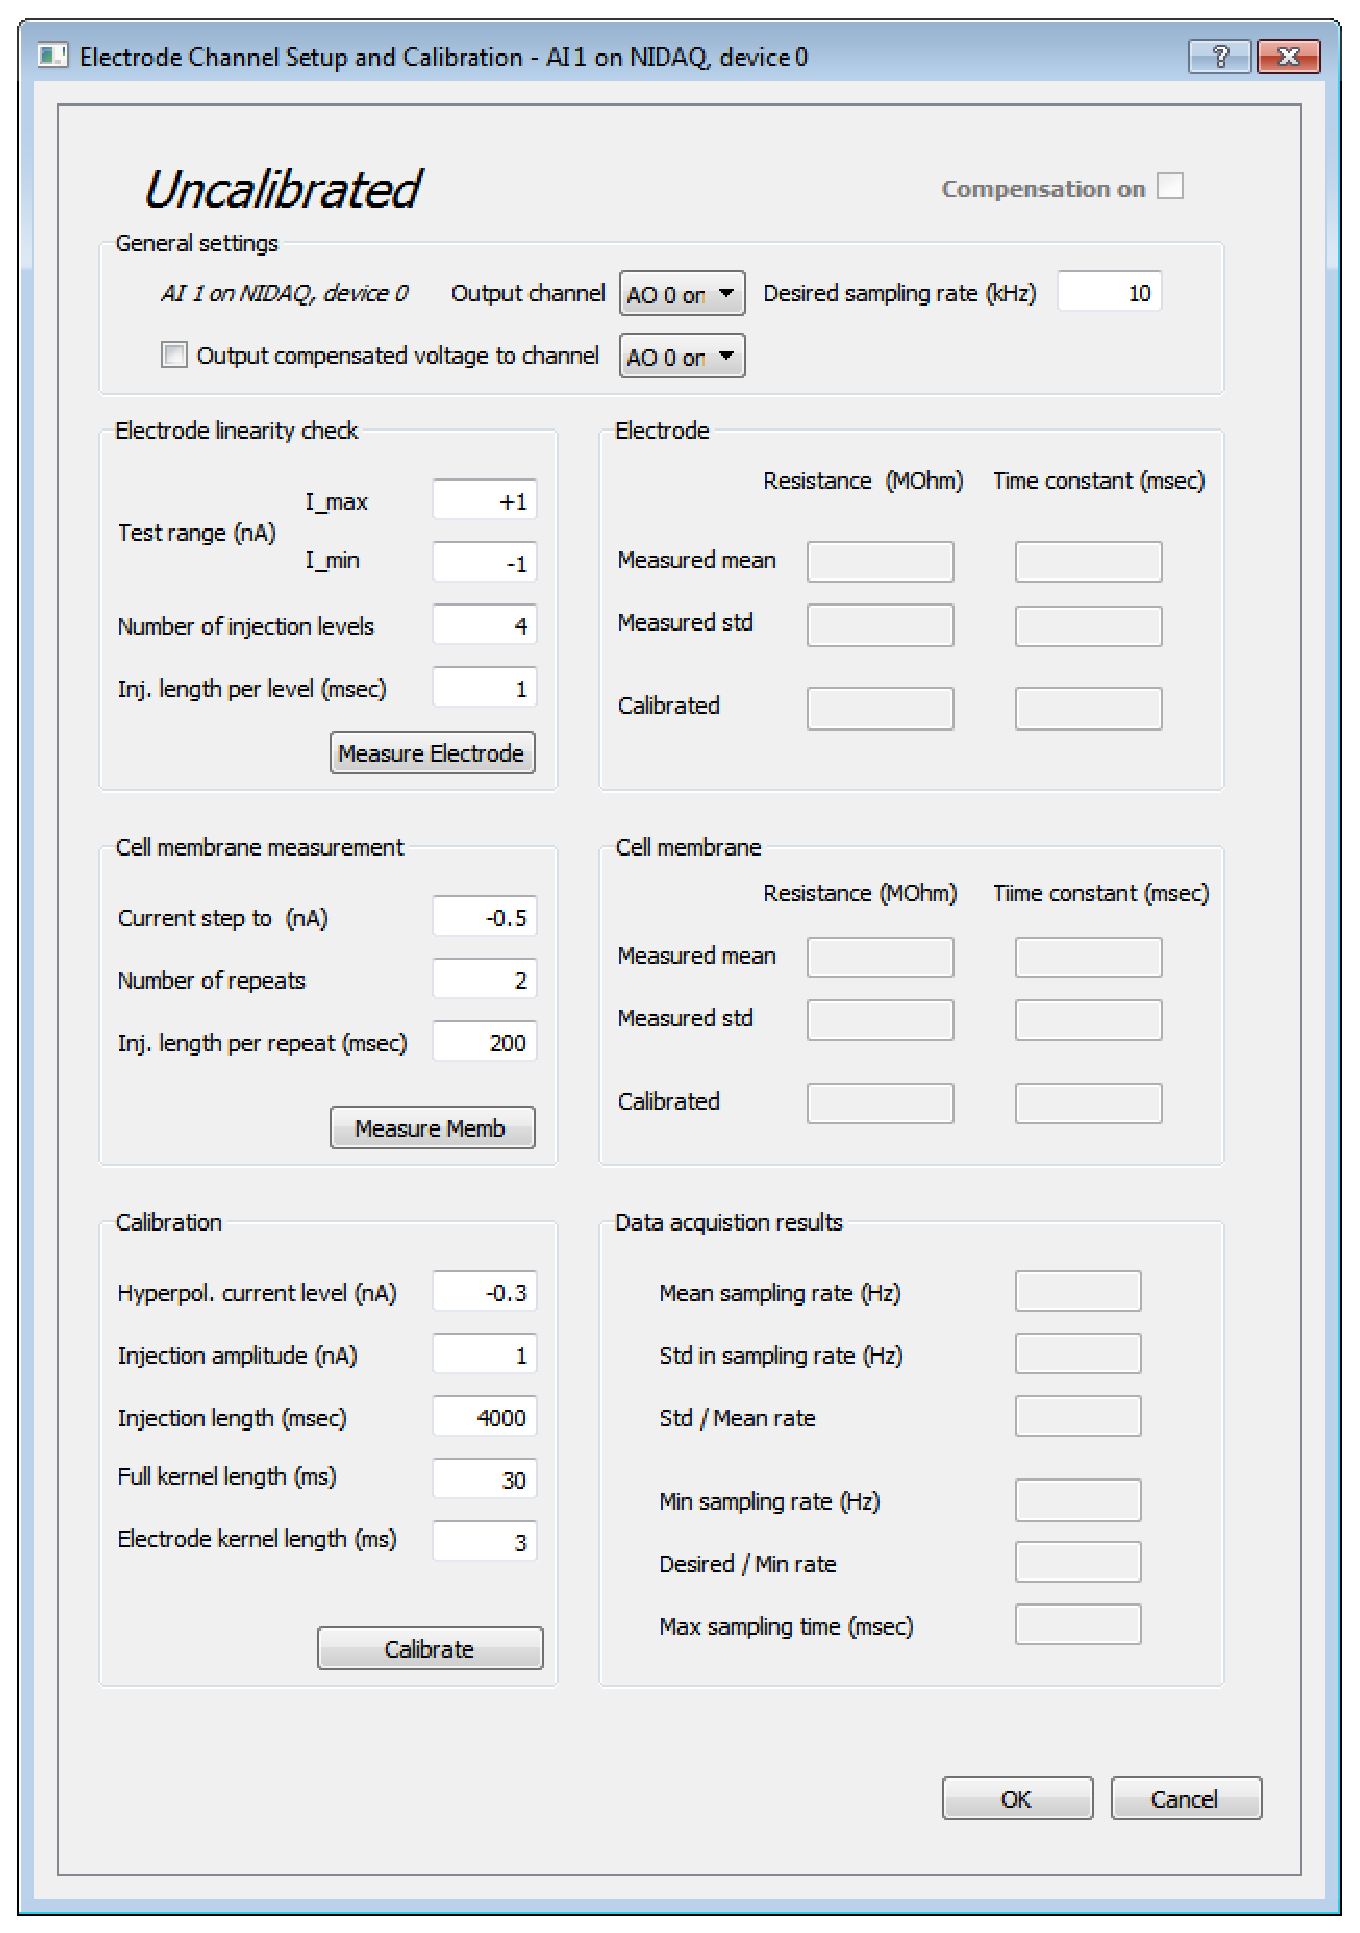
\includegraphics[scale=0.6]{elecCalibDialog}

The calibration dialog is reached through the input channel setup dialog.
The control and result elements are the following:  
\begin{myitem}
\item Information line: Each page has a text line on the top (saying
  \emph{Uncalibrated} on the included picture) to provide some basic
  information about the calibration process for the user. 
\item \emph{Compensation on}: after calibration, this checkbox allows the
  user to turn the compensation on and off on the corresponding electrode.
\end{myitem}
\emph{General settings}: This panel contains the settings that
  apply to all the available features (ie. the electrode measurement, the
  membrane measurement and the calibration).
\begin{myitem}
\item \emph{Output channel}: The output channel assigned to the
  electrode, must be one of the active output channels.
\item \emph{Output compensated voltage to channel} Check and select a different
  channel to copy the compensated voltage to. This can be used to record the
  voltage actually used by StdpC on a separate machine, for example.
\item \emph{Desired sampling rate}: The sampling frequency that StdpC will
  aim to keep during the calibration or the electrode/membrane measurement.
\end{myitem}
\emph{Electrode linearity check}: This panel contains the settings specific for
  the electrode measurement feature.
\begin{myitem}
\item \emph{I\_max}: Maximal current level injected into the electrode.
\item \emph{I\_min}: Minimal current level injected into the electrode.
\item \emph{Number of injection levels}: Number of current levels
  injected during electrode measurement. The current levels are equally
  spaced between the maximal and minimal levels, with the limits
  included. For example, if I\_max = 1 nA, I\_min = -1 nA and \emph{Number of
  current levels} = 4, then the current levels to be injected are $I_1 =
  -1 nA, I_2 = -1/3 nA, I_3 = +1/3 nA, and I_4 = +1 nA$. Zero current level
  is always skipped.
\item \emph{Inj. length per level}: defines how long the injection of each
  current level lasts. 
\item \emph{Cell membrane measurement}: This panel contains the settings specific for
  the cell membrane measurement feature. See also \emph{General settings}. 
\item \emph{Current step to}: Sets the current step at which the cell
  properties will be measured. Negative current steps are highly
  recommended, as depolarization increases the chance that active membrane
  phenomena, like spiking, will disrupt the measurement of passive membrane
  properties. 
\item \emph{Number of repeats}: defines how many time the above current level
  will be injected into the cell. Higher repeat numbers give numerical
  stability to the measurement, but only if no spike has occured during any
  of the injections. 
\item \emph{Inj. length per repeat}: defines how long each injection will
  lasts. Also defines the recovery time in between current level injections. 
\end{myitem}
\emph{Calibration}: This panel contains the settings specific for
  the electrode electrode calibration feature.
\begin{myitem}
\item \emph{Hyperpol. current level}: allows for the injection of a certain
  constant level of  hyperpolarization current into the cell during the
  whole duration of the calibration in order to minimize the number of
  spikes occurring during calibration. High hyperpolarization levels
  (ie. above -1nA) are not favourable, as they can remarkably change the electrode 
  characteristics.
\item \emph{Injection amplitude}: the amplitude of the injected
  white noise current signal. Setting 1 nA here usually means a good
  tradeoff between reaching a high signal-to-noise ratio and avoiding
  driving the cell into 
  an active state (like spiking) in the same time. Always make sure that
  the DAQ hardware allows for the issuing of this current level (both to
  positive and negative levels).
\item \emph{Injection length}: defines how long the current injection during
  the calibration phase lasts. In most cases, a 4-5 second long calibration
  is sufficient to acquire statistically significant amount of data for the
  electrode parameter calculation.   
\item \emph{Full kernel length}: one of the crucial parameters of the AEC
  technique. A rule of thumb is to set it to one or two times of the time constant of
  the membrane. After cell membrane measurement StdpC automatically
  fills this field, however, as the membrane property measurement can be
  quite imprecise in some cases (huge cell, changing electrode properties
  or spiking activity), always check that it is somewhere in between 30 and
  60 ms before issuing the calibration command.
\item \emph{Electrode kernel length}: the other very important parameter for
  the calibration. A rule of thumb here is to set it to 10 times of the
  time constant of the electrode, but to no more than 5ms. After electrode
  measurement StdpC automatically fills this field, however, always
  check that it is somewhere in between 1 and 5 ms before issuing the
  calibration command.
\end{myitem}



\section{Saving of experiment data} \label{datasaving}

StdpC allows saving experiment data to disk.
The user can choose between binary and ASCII data formats, pick
any subset of the active channels (see Section \ref{inchnconfig} and
\ref{outchnconfig}), set the data saving frequency and select a file which the
experiment data will be saved into. After starting the dynamic clamp, in
each clamping cycle the software decides whether it is time to write samples
to file by comparing the last saving time and the current time. This way the
saving frequency is quasi independent of the dynamic clamping
frequency.\\
In ASCII mode, when a data saving occurs, a new line is added to the
data file obeying the following pattern:
\begin{equation*}
Time\_stamp\ \ \ Input\_chnl\_1
\ \ \ ...\ \ \ Input\_chnl\_n\ \ \  Output\_chnl\_1\ \ \ ...\ \ \ Output\_chnl\_n  
\end{equation*}

Please be aware, that, as no offline compression is implemented in the
current version, StdpC can generate huge data files during long
experiments. The size of the saved data can be reduced by
\begin{myitem} 
\item choosing binary format rather than ASCII
\item decreasing the saving frequency
\item only saving the channels which are going to be important for data
  post-processing and analysis
\end{myitem}

For a simple comparison, the simulation of a gap junction (electrical
synapse) between two neurons produces about 30 MByte/minute data if the
user wants to save all the four channels (2 input and 2 output channels
+ the extra time stamp) at 10kHz frequency in ASCII mode, while the same
experiment produces about 3.6 MByte/minute data in case the user only saves the
membrane voltages of the two cells (2 input channels + the extra time
stamp) at 5kHz in binary mode. 
Having finished the experiment, the user can load the experiment data file
into any data analysis platform they prefer (Matlab, R, Octave, Scilab,
etc) for offline processing and analysis of the data.


\noindent
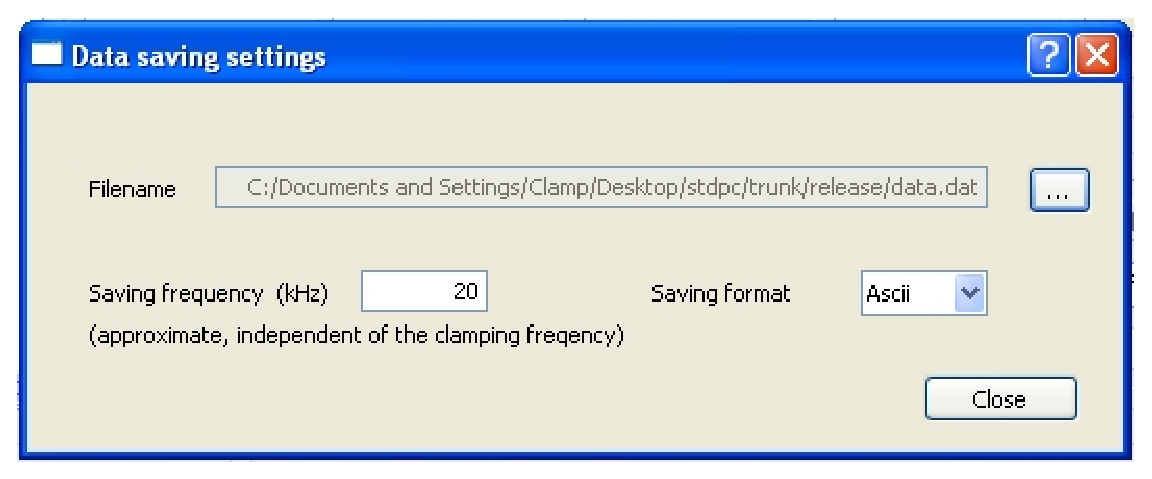
\includegraphics[scale=0.6]{dataSavingDialog}\\

\noindent
The configuration settings on the \emph{Data saving settings} dialog are
the following:
\begin{myitem}
\item Saving frequency: sets the target frequency of data saving.
\item Filename: Indicates the name of the file (ASCII mode) or the directory (binary mode) where data
will be saved. Use placeholders as indicated. Year (\%Y) and consecutive numbers (\%n) are four digits,
all other fields are two digits. Consecutive numbering respects any existing files; if e.g. there are
already files named ``data\_0001.dat'' and ``data\_0004.dat'' in the same location, StdpC will write to
a new file named ``data\_0005.dat'' on the next clamping run.
\item ASCII format: Writes the output as a text file. The first line of the file is a header with the
given header prefix, labelling the columns of data. Each subsequent row is a snapshot of the data in
the chosen channels, at the time (in seconds after clamp cycle initiation) indicated in the first column.
Columns are separated with the character(s) specified in the ``Field separator'' input.
\item Binary format: Instead of writing to a single file, the given filename is interpreted as a directory
name. In this directory, each saved channel is saved to a separate file, along with a file containing
the time stamps. In addition to the raw data, a file named ``meta.json'' is deposited in the same
directory, describing the data set in JSON format.
\end{myitem}


\section{User feedback} 
Please do give feedback if you found the software useful, buggy, or
have general comments or questions. Please send correspondence through
GitHub or directly to T.Nowotny@sussex.ac.uk.
If you are interested in contributing to the future development please
do not hesitate to contact me as well.  
 
\section{Acknowledgements} 
 
The StdpC software would not exist without the early dynamic clamp
versions developed by Reynaldo D. Pinto and I (TN) am grateful to him for supplying the source code for further
development back then. We are also grateful to both Attila Sz\"ucs and Naoki Kogo for their excellent
suggestions for improving and extending the software and their tireless
testing of new and buggy versions.

\bibliographystyle{apalike}
\bibliography{master}
\end{document}
